%%%%%%%%%%%%%%%%%%%%%%%%%%%%%%%%%%%%%%%%%%%%%%%%%%%%%%%%%%%%%%%%%%%%%%%%%%%%%%%%
%2345678901234567890123456789012345678901234567890123456789012345678901234567890
%        1         2         3         4         5         6         7         8

\documentclass[letterpaper, 10 pt, conference]{ieeeconf}  % Comment this line out if you need a4paper

%\documentclass[a4paper, 10pt, conference]{ieeeconf}      % Use this line for a4 paper

\IEEEoverridecommandlockouts                              % This command is only needed if
                                                          % you want to use the \thanks command

\overrideIEEEmargins                                      % Needed to meet printer requirements.

%In case you encounter the following error:
%Error 1010 The PDF file may be corrupt (unable to open PDF file) OR
%Error 1000 An error occurred while parsing a contents stream. Unable to analyze the PDF file.
%This is a known problem with pdfLaTeX conversion filter. The file cannot be opened with acrobat reader
%Please use one of the alternatives below to circumvent this error by uncommenting one or the other
%\pdfobjcompresslevel=0
%\pdfminorversion=4

% See the \addtolength command later in the file to balance the column lengths
% on the last page of the document

% The following packages can be found on http:\\www.ctan.org
%\usepackage{graphics} % for pdf, bitmapped graphics files
%\usepackage{epsfig} % for postscript graphics files
%\usepackage{mathptmx} % assumes new font selection scheme installed
%\usepackage{times} % assumes new font selection scheme installed
%\usepackage{amsmath} % assumes amsmath package installed
%\usepackage{amssymb}  % assumes amsmath package installed

\usepackage{amsmath}
\usepackage{amssymb}
\usepackage{graphicx}
\usepackage{url}
\usepackage{placeins}
\usepackage{balance}
\usepackage{bm}
\usepackage{multirow}
\usepackage{booktabs}

\usepackage[
    pagebackref,
    breaklinks,
    colorlinks=true,
    linkcolor=red,
    citecolor=red,
    filecolor=red,
]{hyperref}
\title{Which Trajectory Is Safer? Learning Future Risk for Autonomous Driving
}


% \author{Albert Author$^{1}$ and Bernard D. Researcher$^{2}$% <-this % stops a space
% \thanks{*This work was not supported by any organization}% <-this % stops a space
% \thanks{$^{1}$Albert Author is with Faculty of Electrical Engineering, Mathematics and Computer Science,
%         University of Twente, 7500 AE Enschede, The Netherlands
%         {\tt\small albert.author@papercept.net}}%
% \thanks{$^{2}$Bernard D. Researcheris with the Department of Electrical Engineering, Wright State University,
%         Dayton, OH 45435, USA
%         {\tt\small b.d.researcher@ieee.org}}%
% }
\author{Anonymous Authors}

\begin{document}



\maketitle
\thispagestyle{empty}
\pagestyle{empty}


%%%%%%%%%%%%%%%%%%%%%%%%%%%%%%%%%%%%%%%%%%%%%%%%%%%%%%%%%%%%%%%%%%%%%%%%%%%%%%%%
\begin{abstract}

Collision rate remains the dominant metric for evaluating trajectory safety, yet as planners increasingly avoid collisions outright, 
it reveals little about the safety differences among trajectories that remain collision-free. 

% Bo Yu 上面整个一句话的中间的部分读起来有点别扭，我下面换了个写完，你可以看看哪个好点。
% Collision rate is the standard metric for trajectory safety, yet it is binary and coarse: once planners avoid collisions in nearly all cases, it saturates and offers no signal about how safe a collision-free trajectory actually is.

We introduce \textbf{FutureRisk}, a metric that scores the \emph{latent future risk} of a trajectory from its own realized future interactions, whether logged from human driving or rolled out by a policy in closed-loop simulation, producing a continuous score that distinguishes collision-free trajectories by how closely and how persistently they approached an unsafe interaction state. At its core, a \textbf{Context-Adaptive Risk Model (CARM)} replaces fixed, hand-crafted TTC-style thresholds with a learned, context-dependent safety criterion, while remaining bounded around an interpretable, closed-form geometric prior. The resulting score is continuous, interpretable, and directly comparable across trajectories on matched scenarios, enabling fine-grained safety evaluation beyond binary collision outcomes. 

% bo yu
% 感觉上面的这部分可以改成，Experiment results show that the proposed latent future risk and its corresponding CARM can achieve .... 从实验结果出发比较好，而不是重复上面的论述，因为ocontinuous, intepretable 已经在上面出现论述过了。用实验结果去论证上面提到过的比较好

%最后可以加一句升华：By exposing near-miss behavior that collision rate alone would deem safe, FutureRisk helps identify hazardous planning behavior before it reaches public roads, supporting the safer deployment of autonomous driving systems. 当然也可以更简略一点最后一句
\end{abstract}


%%%%%%%%%%%%%%%%%%%%%%%%%%%%%%%%%%%%%%%%%%%%%%%%%%%%%%%%%%%%%%%%%%%%%%%%%%%%%%%%


\section{Introduction}

%Recent planning systems have achieved substantial improvements in collision avoidance, resulting in increasingly low collision rates \cite{hamidaoui2025survey}, and this very success is what exposes the limits of collision rate as a safety metric: once collisions become rare events, collision rate alone increasingly fails to distinguish planners by the safety they actually deliver. Observing only whether a collision or near-collision eventually occurs is insufficient to evaluate whether an automated driving system maintains a continuously safe operating state \cite{weng2020mprism}. Collision occurrence therefore provides a direct and critical measure of safety failure, but as an outcome-based metric, it reveals little about the safety differences among trajectories that ultimately remain collision-free \cite{jiang2025interactive, cui2025unified}. A collision-free outcome does not necessarily imply that a trajectory is sufficiently safe: some may maintain ample safety margins throughout the interaction, whereas others may encounter safety-critical situations with limited room for recovery or avoid collisions only because surrounding agents respond favorably. These distinctions are largely obscured by collision-based evaluation, limiting its ability to discriminate among trajectories with substantially different safety profiles.

% boyu (第一段)
% Recent planning systems have achieved substantial improvements in collision avoidance, resulting in increasingly low collision rates, a commonly used safety evaluation metric to measure whether a collision or near-collision eventually occurs. Such coarse-grained evaluation metrics can produce overly optimistic safety assessments, potentially leading researchers and practitioners to underestimate residual risks and lower their vigilance toward autonomous driving safety. When such risks materialize in real-world deployment, the consequences can be catastrophic and irreversible. In reality, a collision-free outcome does not necessarily imply that a trajectory is sufficiently safe: some may maintain ample safety margins throughout the interaction, whereas others may encounter safety-critical situations with limited room for recovery or avoid collisions only because surrounding agents respond favorably. These distinctions are largely obscured by collision-based evaluation, limiting its ability to discriminate among trajectories with substantially different safety profiles.

% xuewen

Recent planning systems have achieved substantial improvements in collision avoidance, resulting in increasingly low collision rates \cite{hamidaoui2025survey}. Nevertheless, collision occurrence, which often summarized as a collision rate, remains a dominant safety measure. This binary outcome reveals little about the safety differences among trajectories that ultimately remain collision-free \cite{weng2020mprism} and may therefore produce overly optimistic assessments by obscuring risks that do not materialize as collisions \cite{jiang2025interactive, cui2025unified}. In practice, a collision-free trajectory is not necessarily a sufficiently safe one: some trajectories maintain ample safety margins throughout an interaction, whereas others enter safety-critical situations with limited room for recovery or avoid collisions only because surrounding agents respond favorably. Collision-based evaluation cannot distinguish among these substantially different safety profiles.



%This is not a new concern -- it has been raised repeatedly, from several independent angles, at least since the early 2020s, and a range of alternative safety metrics has emerged to address it \cite{arun2021systematic}. As we discuss in Sec.~\ref{sec:related}, these attempts typically satisfy only one of two desirable properties: formula-based criteria such as TTC remain interpretable but rely on fixed, scenario-agnostic assumptions \cite{westhofen2023criticality}, while learning-based alternatives adapt to scenario context but forfeit the closed-form interpretability that a formula provides \cite{lu2022learning}. Because each line of work lacks what the other provides, we seek a safety metric that combines the interpretability of a formula-based criterion with the scenario-dependent adaptivity of a learned one.

% boyu （第二段）
% In recent years, researchers have increasingly recognized this concern and have sought to address it. As we discuss in Sec.~\ref{sec:related}, existing criteria face a persistent trade-off between two desirable properties: interpretability and context adaptivity. Formula-based criteria such as TTC are interpretable by construction, yet they encode fixed, scenario-agnostic assumptions that do not transfer across driving contexts \cite{westhofen2023criticality}. Learning-based alternatives adapt to scenario context, but they abandon the closed-form structure that made such criteria interpretable in the first place \cite{lu2022learning}. To our knowledge, no existing criterion achieves both.

%xuewen

To move beyond binary collision outcomes, prior work has introduced prospective safety and criticality criteria that quantify proximity to hazardous interactions \cite{arun2021systematic}. However, existing criteria exhibit a persistent trade-off between two desirable properties: interpretability and context adaptivity. Formula-based criteria are interpretable by construction, but typically rely on fixed assumptions and thresholds that may not adequately reflect differences across driving contexts \cite{westhofen2023criticality}. Learning-based alternatives can adapt to contextual variations, but often lack the explicit closed-form structure that makes their outputs physically interpretable \cite{lu2022learning}. To our knowledge, existing criteria do not explicitly combine both properties within a unified metric.

% xuewen
Together, these gaps motivate us to reconsider how the safety of an executed trajectory should be characterized beyond its eventual collision outcome. A more informative safety metric should not only distinguish different levels of risk among collision-free trajectories, but also remain interpretable while adapting its safety criterion to the interaction context. Drawing on prior notions of prospective safety and criticality \cite{wang2021review}, we characterize risk at each point along an executed trajectory by how closely and how persistently its subsequent evolution approaches an unsafe interaction state. This risk is \emph{future} with respect to the evaluated point, but is computed retrospectively from the future evolution that actually occurred. It is \emph{latent} because it may remain hidden when the interaction does not ultimately result in a collision. We therefore refer to this quantity as \textbf{latent future risk}. Quantifying latent future risk places collision-free trajectories along a continuous spectrum of safety, addressing the limitations of binary collision outcomes; doing so through an interpretable yet context-adaptive criterion further resolves the trade-off exhibited by existing criticality measures. This leads to the central question of this work: \textbf{How can the latent future risk of an executed trajectory be quantified in a manner that is both interpretable and adaptive to scenario context?}

\begin{figure}[t]
\vspace{-5mm}
\centering
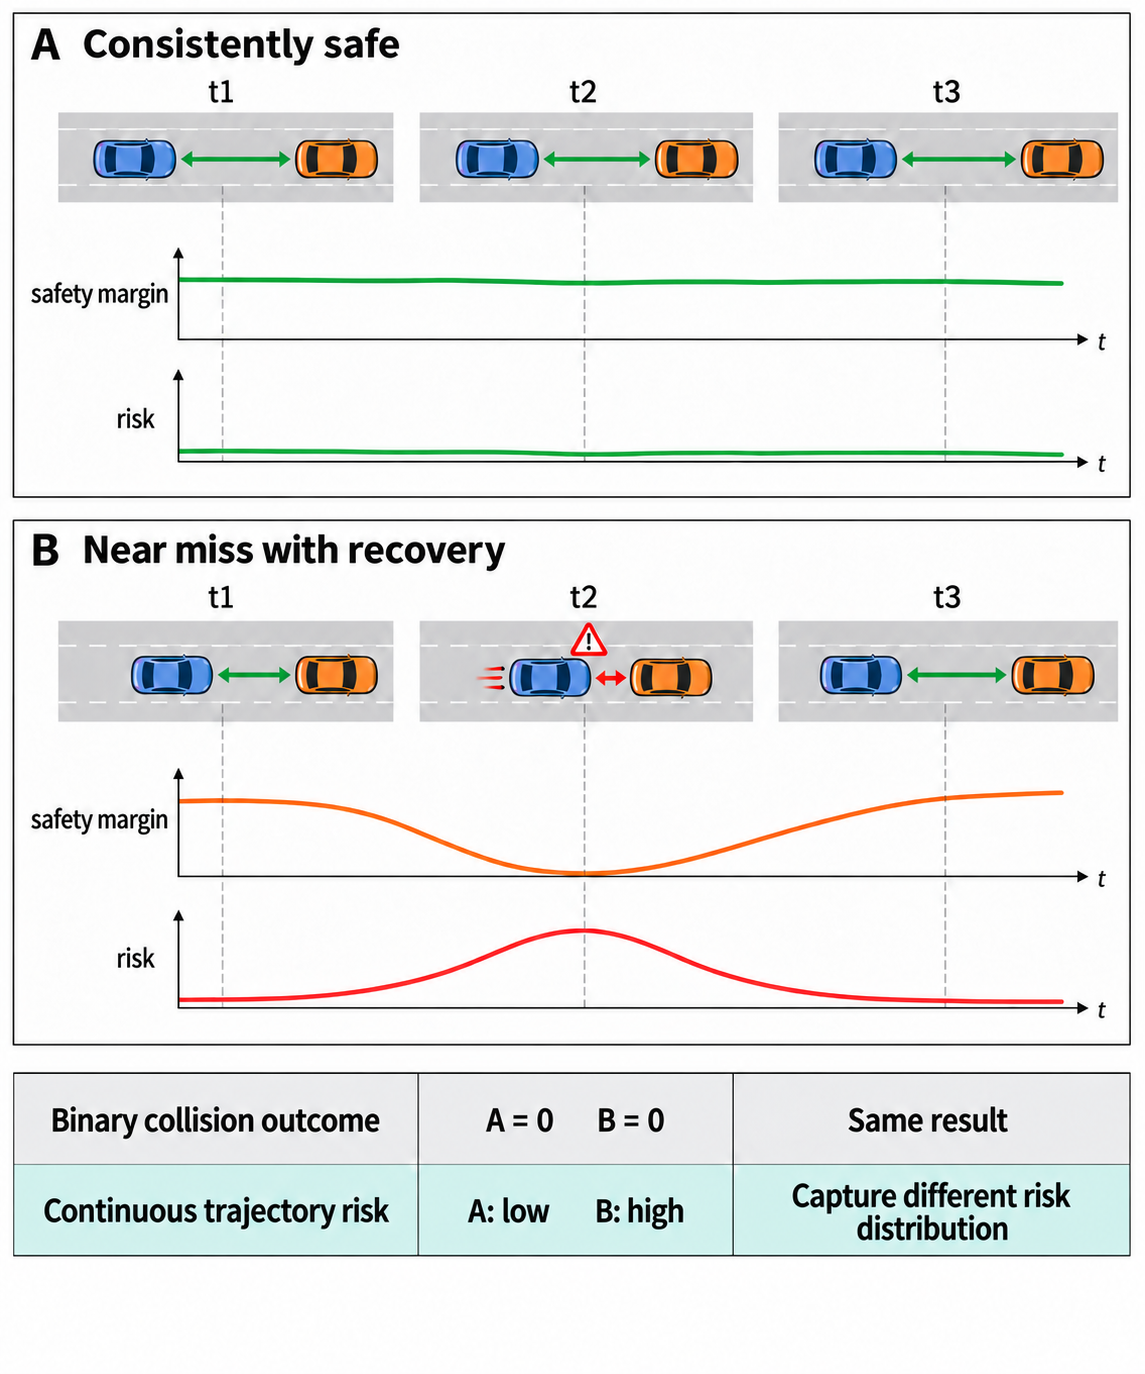
\includegraphics[width=2.5in]{figures/futurerisk-margin-evolution-centered.png}
\vspace{-11mm}
\label{fig:futurerisk-margin-evolution}
\end{figure}


%This motivates a more fine-grained evaluation of trajectory safety beyond whether a collision eventually occurs. Drawing on prior notions of prospective safety and criticality \cite{wang2021review}, we consider how closely and how persistently an already-executed trajectory approaches unsafe interaction states over its own observed future evolution, together with the remaining margin to maintain or recover a safe state. We refer to this trajectory-level notion as \textbf{latent future risk}. Latent future risk captures how risk develops throughout future interactions and places collision-free trajectories along a continuous spectrum of safety. This leads to a fundamental question: \textbf{how can we quantify the latent future risk of an executed trajectory to enable fine-grained safety evaluation beyond collision outcomes?}

% boyu （第三段）
% These limitations motivate a safety metric that evaluates trajectories beyond binary collision outcomes while combining the interpretability of a formula-based criterion with the scenario-dependent adaptivity of a learned one. Drawing on prior notions of prospective safety and criticality \cite{wang2021review}, we instead ask, at each point along an executed trajectory, how closely and how persistently its subsequent evolution approaches an unsafe interaction state. Because this risk is assessed retrospectively from the trajectory's own realized future and need not materialize as a collision, we refer to it as \textbf{latent future risk}. Quantifying it would place collision-free trajectories along a continuous spectrum of safety rather than collapsing them into a single outcome. This raises the central question of this work: \textbf{how can the latent future risk of an executed trajectory be quantified in a way that is both interpretable and adaptive to scenario context?}

%To this end, we propose \textbf{FutureRisk}, a metric for the latent future risk of a trajectory, computed from its own realized future interactions -- whether logged from human driving or rolled out by a policy in closed-loop simulation. At its core, our \textbf{Context-Adaptive Risk Model (CARM)} learns context-dependent safety criteria from the observed interaction and geometry-aware 3D-TTC, replacing hand-crafted rules and universal TTC thresholds with an adaptive and interpretable assessment of trajectory risk, while remaining bounded around the same closed-form geometric quantities that make a fixed criterion interpretable in the first place. The resulting continuous and interpretable risk score reveals fine-grained safety differences among trajectories sharing the same collision outcome, and supports both auditing the safety profile of trajectories already produced by a planner or by human drivers, and comparing methods by contrasting the risk-score distributions of their trajectories on matched scenarios. Operating directly on trajectories without requiring planner-specific internal representations, FutureRisk can serve as a general safety evaluation metric across different planning systems and data sources. 

% boyu （第四段）
% 这一段感觉这样写是不是更好？To this end, we propose \textbf{FutureRisk}, a metric that quantifies the latent future risk of a trajectory from its own realized future interactions, whether logged from human driving or rolled out by a policy in closed-loop simulation. At its core, our \textbf{Context-Adaptive Risk Model (CARM)} starts from a closed-form geometric criticality measure (a geometry-aware 3D time-to-collision, Sec.~\ref{sec:method}) and learns how the safety threshold on this measure should vary with the observed interaction context. This replaces hand-crafted rules and universal TTC thresholds with a context-adaptive criterion, while the learned criterion remains bounded around the closed-form prior, so that every score retains a direct geometric interpretation. The resulting continuous risk score exposes fine-grained safety differences among trajectories that share the same collision outcome. It supports auditing the safety profile of individual trajectories as well as comparing planning methods through the distributions of their scores on matched scenarios. Because FutureRisk operates directly on trajectories and requires no planner-specific internal representations, it applies uniformly across planning systems and data sources.

% boyu （第四段最后一部分）
% 感觉上面一段最后一部分得说明一下实验效果，才能更strongly support上面的论述，有可能的模版如下，但是根据你自己的实验结果好好写一下会更好。Experiments on [dataset A] and [closed-loop benchmark B] show that FutureRisk separates collision-free trajectories that collision rate and fixed-threshold TTC treat as equivalent, ranks [N] state-of-the-art planners consistently with [human judgment / downstream safety outcomes / expert annotations], and yields risk attributions that align with the underlying interaction geometry.

To this end, we propose \textbf{FutureRisk}, a metric that quantifies the latent future risk of an executed trajectory from its realized future interactions. At its core, our \textbf{Context-Adaptive Risk Model (CARM)} starts from a geometry-aware 3D time-to-collision (TTC), which provides a closed-form physical measure of geometric criticality, and learns how the corresponding safety criterion should vary with the observed interaction context. CARM thereby replaces universal TTC thresholds and hand-crafted scenario rules with a context-dependent criterion, while retaining the closed-form measure as a physical anchor for interpretation. FutureRisk uses this criterion to capture both the severity and persistence of risk along the realized trajectory. The resulting continuous score reveals fine-grained safety differences among trajectories that share the same collision outcome, supporting trajectory-level safety auditing as well as method-level comparison through score distributions over matched scenarios. 
% Because FutureRisk operates directly on realized trajectories and requires no planner-specific internal representations, it can be applied uniformly across planning systems and data sources.

Our main contributions are summarized as follows:

\begin{itemize}

\item We introduce \textbf{FutureRisk}, a continuous trajectory-level safety metric that assesses risk from interactions with surrounding agents. Beyond binary collision outcomes, FutureRisk provides a fine-grained assessment of interaction risk to distinguish trajectories that remain collision-free but exhibit different levels of safety.

\item We develop the \textbf{CARM}, which combines critical-event timing with a context-dependent safety-time distribution whose median is constrained around a closed-form physical prior. A two-stage training scheme first learns this structured risk estimate and then fits a bounded logit residual with the structured branch frozen, allowing further adjustment while explicitly limiting its effect on the final score.

\item We evaluate FutureRisk through its agreement with collision outcomes, its discrimination among collision-free trajectories with different safety margins, and its zero-shot transfer across datasets. Qualitative analyses further examine how the metric responds to observed interaction dynamics.

\end{itemize}

\section{Related Work}
\label{sec:related}

\textbf{Beyond collision rate.} Recent planning systems have driven collision rates increasingly low \cite{hamidaoui2025survey}, which has sharpened rather than resolved a long-standing concern: collision occurrence is a direct measure of safety failure, but as an outcome-based metric it reveals little about the safety differences among trajectories that ultimately remain collision-free \cite{jiang2025interactive, cui2025unified}. Prior work on real-time safety metrics has argued directly that observing eventual collisions or near-collisions is insufficient to evaluate whether an automated driving system maintains a continuously safe operating state \cite{weng2020mprism}. This coarseness persists even in more sophisticated evaluation frameworks: nuPlan's Closed-Loop Score blends progress, comfort, and minimum TTC into a continuous value, yet still gates that value multiplicatively to zero on any at-fault collision or off-road event, so its underlying safety judgment collapses back to a binary pass/fail the moment a violation occurs \cite{caesar2021nuplan}. The Waymo Open Sim Agents Challenge shows this can be exploited outright: a trivially static policy can drive collision rate to zero without being safe \cite{montali2023wosac}. Together, these findings motivate safety metrics that assign continuous, fine-grained scores to trajectories rather than relying on sparse collision outcomes.

\textbf{Rule-based safety criteria.} One response is to define safety through closed-form, rule-based criteria over kinematic or geometric quantities, such as time-to-collision (TTC), post-encroachment time, and deceleration rate to avoid a crash \cite{arun2021systematic, wang2021review}, or explicit safety envelopes such as Responsibility-Sensitive Safety \cite{shalevshwartz2017rss}. Because these criteria are given by an explicit formula, they are transparent, auditable, and reliable in the sense that their behavior can be verified independently of any training data. However, their thresholds and assumptions are hand-specified once and then applied uniformly, without regard for the specific scene or object being evaluated. Westhofen \emph{et al.}'s systematic review of criticality metrics shows the resulting cost: no single formulation is valid across all scenario types, and even a continuous measure such as TTC is effective for car-following but breaks down at intersections, where single-point kinematics no longer characterize the interaction \cite{westhofen2023criticality}. Rule-based criteria therefore trade flexibility for reliability and interpretability.

\textbf{Data-driven safety criteria.} A complementary line of work learns safety criteria directly from trajectory data instead of specifying them by hand. Lu \emph{et al.} embed sequences of surrogate safety measures such as TTC into a latent space with unsupervised representation learning and identify traffic conflicts by clustering that space, allowing the resulting criterion to reflect patterns in the data rather than a fixed threshold \cite{lu2022learning}. This flexibility comes at the cost of the reliability and interpretability that rule-based criteria offer: the learned criterion no longer corresponds to a verifiable closed-form quantity, and because it is fit to the interaction patterns present in its training data, its behavior on scenes or objects that differ from that distribution is not guaranteed, making generalization to unseen or underrepresented scenarios a central concern for this line of work. FutureRisk is designed to sit between these two extremes: its Context-Adaptive Risk Model learns a scene- and object-dependent safety criterion, as in this line of work, while remaining bounded around the same closed-form geometric quantities used by rule-based criteria, so that the resulting risk score remains anchored to an interpretable formula even as it adapts to context.

\section{Method}
\label{sec:method}

\subsection{Overview}
\label{sec:method_overview}

\begin{figure*}[t]
    \vspace{-5mm}
    \centering
    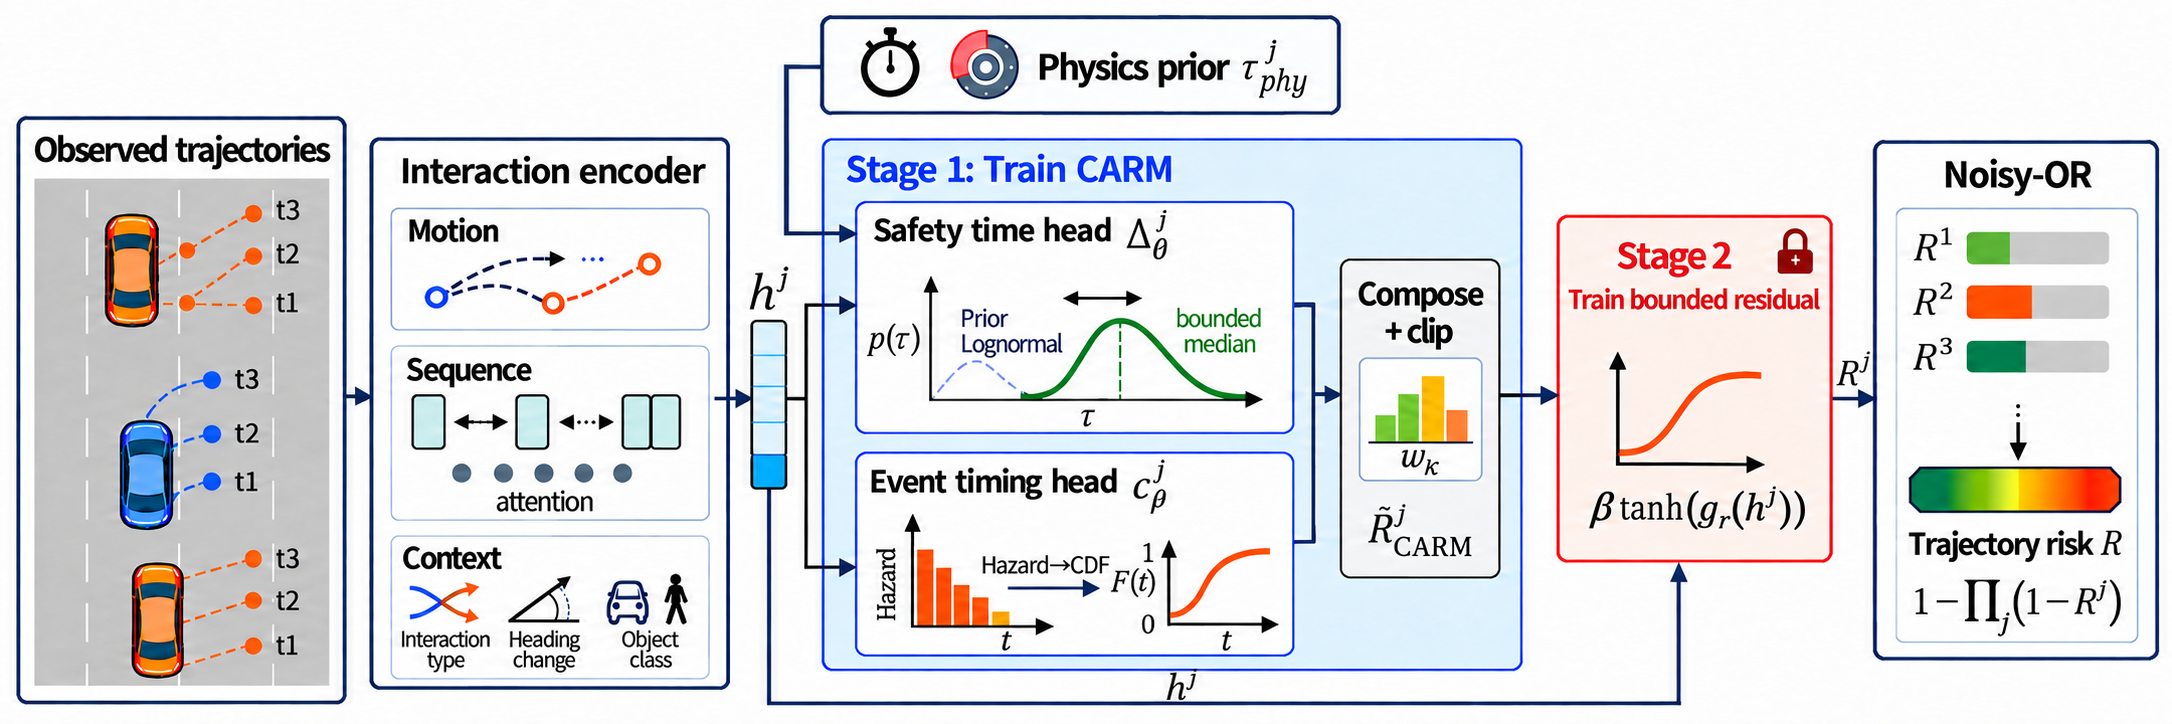
\includegraphics[width=0.8\textwidth]{figures/futurerisk_method.png}
    \caption{Overview of how FutureRisk is computed.}
    \vspace{-6mm}
    \label{fig:futurerisk_method}
\end{figure*}

FutureRisk assigns a continuous risk score to an ego trajectory based on its
interactions with surrounding agents. Let $\bm{\xi}_e$ denote an ego
trajectory over a horizon $H$, and let
$\mathcal{W}^{\mathrm{obs}}=\{\bm{\xi}_j\}_{j=1}^{J}$ denote the trajectories
of $J$ surrounding agents over the same horizon. FutureRisk maps these inputs
to a continuous score
\begin{equation}
R = f_{\mathrm{FR}}\big(\bm{\xi}_e,\mathcal{W}^{\mathrm{obs}}\big)\in[0,1],
\label{eq:future_risk_objective}
\end{equation}
where a larger $R$ means the trajectory approached an unsafe interaction
state more closely, or stayed near one for longer. A binary collision label
assigns the same value to a trajectory that kept a wide margin throughout
and to one that avoided contact by a fraction of a second. But $R$ separates
them. Throughout, time within the horizon is discretized into $K$ bins with
edges $0=b_0<b_1<\dots<b_K=H$; every time-dependent quantity introduced below
is evaluated on this one grid, and $\sigma(\cdot)$ always denotes the
logistic function.

At the core of $f_{\mathrm{FR}}$ is CARM: a risk prediction model with a
learned, context-dependent safety criterion, while remaining bounded
around an interpretable, closed-form physics prior. Concretely, for each
surrounding agent $j$, CARM corrects a structured risk estimate
$\widetilde R_{\mathrm{CARM}}^{j}$ with a further, learned bounded
correction to obtain a per-agent risk $R^{j}$ (Sec.~\ref{sec:bounded_residual}),
and $f_{\mathrm{FR}}$ aggregates these across all agents
(Sec.~\ref{sec:trajectory_aggregation}):
\begin{equation}
\begin{aligned}
R&=1-\prod_{j}\left(1-R^{j}\right),\\[2pt]
R^{j}&=\sigma\!\left(
\operatorname{logit}\big(\widetilde R_{\mathrm{CARM}}^{j}\big)
+
\underbrace{\beta\tanh\!\left(g_r(\bm h^{j})\right)}_{\text{learned, Stage 2}}
\right).
\end{aligned}
\label{eq:future_risk_decomposition}
\end{equation}
Here $\operatorname{logit}(\cdot)$ denotes the inverse of $\sigma(\cdot)$;
$\bm h^{j}$ is a shared representation of the interaction between the ego
and agent $j$, detailed in Sec.~\ref{sec:CARM_Architecture}; $g_r$ is a
learned scalar head reading from $\bm h^{j}$; and $\beta$ is a fixed
constant bounding the magnitude of this Stage-2 correction.
$\widetilde R_{\mathrm{CARM}}^{j}$ is itself built from the two arguments
that $\Gamma$ combines: the first argument is a required-safety-margin
term, namely one raw, closed-form physics quantity plus one learned
correction to it; the second argument is a separately learned, unanchored
quantity for \emph{when} the interaction turns critical
(Sec.~\ref{sec:CARM_Architecture}):
\begin{equation}
\widetilde R_{\mathrm{CARM}}^{j}
=
\Gamma\!\Big(
\underbrace{\tau_{\mathrm{phy}}^{j}}_{\text{raw}}+\underbrace{\Delta_{\theta}^{j}}_{\text{learned, Stage 1}},\ \
\underbrace{c_{\theta}^{j}}_{\text{learned, Stage 1}}
\Big).
\label{eq:carm_score_ingredients}
\end{equation}
$\tau_{\mathrm{phy}}^{j}$ is the one raw, closed-form quantity in this
composition: a physics prior for the required safety margin, summarizing
closing speed, available deceleration, reaction time, and prediction
uncertainty. It is distinct from the geometry-aware 3D-TTC
$\tau_{\mathrm{3D}}^{j}$, which never enters CARM's \emph{forward
computation} at all; $\tau_{\mathrm{3D}}^{j}$ is used only, offline, to
construct the training target that supervises the whole model, as
Sec.~\ref{sec:carm_training} makes precise. Every other quantity above is
a network output. $\Delta_{\theta}^{j}$ is a bounded correction to
$\tau_{\mathrm{phy}}^{j}$. $c_{\theta}^{j}$ is a separate, unanchored term
for \emph{when} the interaction turns critical, realized as a
discrete-time hazard distribution that predicts the probability the
interaction has already turned critical by each time bin; it is
supervised independently, so that criticality is never defined
circularly in terms of the very margin it is combined with. $\Gamma$
composes the two into a single structured estimate.
The Stage-2 correction $\beta\tanh(g_r(\bm h^{j}))$ from
Eq.~\eqref{eq:future_risk_decomposition} then applies a further, equally
free correction on top of it, trained only after the rest of the network
is frozen. Sec.~\ref{sec:carm_training} derives the geometric target that
supervises $R_\theta$, the score $R$ from
Eq.~\eqref{eq:future_risk_decomposition}, viewed as a function of the
model's trainable parameters $\theta$, together with the independent
label that supervises $c_\theta^{j}$, and the two-stage schedule that
trains every piece above.



\subsection{CARM Architecture}
\label{sec:CARM_Architecture}

CARM turns the interaction between the ego and agent $j$ into the
structured estimate $\widetilde R_{\mathrm{CARM}}^{j}$, which is later
corrected by a further bounded residual (Sec.~\ref{sec:bounded_residual}).
Building $\widetilde R_{\mathrm{CARM}}^{j}$ takes four steps: a shared
interaction representation, a physically anchored model of how much
safety time the interaction requires, an independently learned model of
when it turns critical, and a composition of the two into a single
structured risk estimate.

\subsubsection{Interaction Representation}

Every branch below, the safety-time model, the critical-event model, and
the bounded residual introduced separately, reads from a single shared
representation of the interaction between the ego and agent $j$. For ego
trajectory $\bm{\xi}_e$ and agent $j$, the model receives three input
groups: current relative kinematics $\bm{x}_{\mathrm{kin}}^{j}$ (relative
position and velocity, relative heading, closing speed, and each party's
own speed at the current instant), the observed interaction sequence
$\bm{X}_{\mathrm{int}}^{j}$ (relative 3D motion together with a
signed-clearance proxy, the center-to-center distance offset by the sum of
each box's half-diagonal, sampled over the full observed horizon
$[0,H]$), and semantic scene context $\bm{x}_{\mathrm{ctx}}^{j}$ (the
interaction-type distribution, relative-heading statistics, ego's own
heading change, and the agent's object class). The signed-clearance proxy
is a lightweight, differentiable stand-in for an exact oriented-box
overlap test: cheap to evaluate at every bin and smooth enough to
backpropagate through, not the exact geometric quantity a fixed criterion
would use.

A bidirectional recurrent encoder (GRU) with attention pooling
over $\bm{X}_{\mathrm{int}}^{j}$ summarizes the interaction history, while
separate MLPs encode $\bm{x}_{\mathrm{kin}}^{j}$ and
$\bm{x}_{\mathrm{ctx}}^{j}$. The three encodings are concatenated, passed
through a fusion MLP, and layer-normalized:
\begin{equation}
\bm h^{j}
=f_{\mathrm{enc}}\!\left(
\bm{x}_{\mathrm{kin}}^{j},
\bm{X}_{\mathrm{int}}^{j},
\bm{x}_{\mathrm{ctx}}^{j}
\right).
\label{eq:carm_encoder}
\end{equation}
Normalizing this final representation keeps its scale fixed regardless of
what the rest of the encoder settles into during training. Without it, the
single-scalar heads introduced next receive an input whose scale drifts
over training and can saturate the bounded nonlinearities they are passed
through, silently collapsing their dependence on context.

\subsubsection{Physically Anchored Safety-Time Modeling}

The first branch answers how much recovery margin the interaction with
agent $j$ actually requires. It starts from a closed-form physics prior,
\begin{equation}
\tau_{\mathrm{phy}}^{j}
=
\mathrm{clip}\!\left(
t_{\mathrm{react}}+\frac{v_{\mathrm{close}}^{j}}{a_{\mathrm{avail}}}+\epsilon_{\mathrm{unc}},
\ [\tau_{\min},\tau_{\max}]
\right),
\label{eq:phy_prior}
\end{equation}
where $v_{\mathrm{close}}^{j}$ is the closing-speed component along the
current relative bearing, $t_{\mathrm{react}}$ a fixed reaction time,
$a_{\mathrm{avail}}$ an assumed available deceleration, and
$\epsilon_{\mathrm{unc}}$ a constant pad absorbing prediction uncertainty.
All four constants, and the clipping range, are specific to agent $j$'s
object class: a pedestrian's evasive capability, reaction time, and
predictability are nothing like a vehicle's, so $\tau_{\mathrm{phy}}^{j}$
already reflects what kind of agent is being reasoned about before any
learning takes place.

CARM corrects this prior in log-space by a bounded, learned amount,
\begin{align}
\mu_s^{j}
&=\log\tau_{\mathrm{phy}}^{j}
+\underbrace{\Delta_{\max}\tanh\!\left(g_{\mu}(\bm h^{j})\right)}_{\Delta_\theta^j},
\nonumber\\
\sigma_s^{j}
&=\sigma_{\min}+(\sigma_{\max}-\sigma_{\min})
\sigma\!\left(g_{\sigma}(\bm h^{j})\right),
\nonumber\\
T_s^{j}&\sim\operatorname{LogNormal}\!\left(\mu_s^{j},(\sigma_s^{j})^2\right),
\label{eq:adaptive_safe_ttc}
\end{align}
and treats the required safety time as the random variable $T_s^{j}$
rather than a single number. Because $\exp(\mu_s^{j})$ is exactly the
median of a log-normal distribution, the bound $\Delta_{\max}=\log 2$
constrains the median of $T_s^{j}$, not its mean, to lie within a factor
of two of $\tau_{\mathrm{phy}}^{j}$ in either direction: CARM can judge
that half the physically assumed margin already suffices, or that twice
as much is warranted, but nothing more extreme. $\tau_{\mathrm{phy}}^{j}$
is evaluated at every bin edge $b_k$ of the same time bins
$0=b_0<b_1<\cdots<b_K=H$ used throughout, rather than as a single scalar,
so $\mu_s^{j}$ is itself bin-indexed even though the correction
$\Delta_\theta^j$ is a single scalar per agent-instance applied uniformly
across every bin.

\subsubsection{Critical-Event-Time Modeling}

The second branch answers when the interaction with agent $j$ turns
critical: the term the overview denotes $c_\theta^j$. Rather than a single
scalar, CARM predicts a full discrete-time hazard distribution over the
same $K$ bins. For each bin $k$, a head produces a conditional hazard,
$q_k^j=\sigma(g_k^{\mathrm{evt}}(\bm h^j))$, the probability that the
critical event falls in bin $k$ given that it has not already occurred in
an earlier bin. The event probability mass and cumulative distribution
follow the standard discrete-time survival parameterization,
\begin{equation}
\begin{aligned}
p_k^j&=q_k^j\prod_{\ell<k}(1-q_\ell^j),
&F_k^j&=\sum_{\ell=1}^{k}p_\ell^j,
\end{aligned}
\label{eq:event_time_distribution}
\end{equation}
so $F_k^j$, evaluated across all $k$, is exactly $c_\theta^j$: the
probability that the interaction has already turned critical by bin $k$.
Because $\sum_{k=1}^{K}p_k^j=1-\prod_{\ell=1}^{K}(1-q_\ell^j)$, the
complementary probability $\prod_{\ell=1}^{K}(1-q_\ell^j)=1-F_K^j$ is
exactly the probability that no critical event occurs anywhere within the
observed horizon, so a genuinely safe interaction is represented on its
own terms rather than forced into an artificial event bin. This
prediction has no closed-form anchor of its own; how its training label
is constructed, independently of the safety-time branch above, is
addressed separately.

\subsubsection{Structured Risk Composition}

The two branches combine into
$\widetilde R_{\mathrm{CARM}}^{j}=\Gamma(\tau_{\mathrm{phy}}^{j}+\Delta_\theta^j,\,c_\theta^j)$
from Eq.~\eqref{eq:carm_score_ingredients}. Writing $\Phi$ for the
standard normal CDF, the safety-time distribution assigns each bin a
probability mass
\begin{equation}
\begin{aligned}
\Pr(b_{k-1}<T_s^j\le b_k) &= \Phi\!\left(\tfrac{\log b_k-\mu_s^j}{\sigma_s^j}\right)-\Phi\!\left(\tfrac{\log b_{k-1}-\mu_s^j}{\sigma_s^j}\right), \\
\Pr(T_s^j> b_K) &= 1-\Phi\!\left(\tfrac{\log b_K-\mu_s^j}{\sigma_s^j}\right),
\end{aligned}
\end{equation}
using $\mu_s^{j},\sigma_s^{j}$ at their own bin from
Eq.~\eqref{eq:adaptive_safe_ttc}. Because $\tau_{\mathrm{phy}}^j$, and
therefore $\mu_s^j$, is itself evaluated per bin, each of these $K+1$
quantities is a CDF difference of a distribution parameterized
\emph{at that bin}, not of one distribution shared across every bin:
each is individually a valid probability in $[0,1]$, but, unlike disjoint
slices of a single CDF, they are not guaranteed to sum to exactly one.
$\Gamma$ combines them with the critical-event probability $F_k^j$ as the
value attached to each bin, approximating the expectation of the
critical-event CDF at the time the interaction's safety margin runs out,
\begin{align}
R_{\mathrm{CARM}}^{j}
&\approx\mathbb E_{T_s^j}\!\left[F_{\mathrm{evt}}^{j}(T_s^j)\right]
\nonumber\\
&=\sum_{k=1}^{K}F_k^j\Pr(b_{k-1}<T_s^j\le b_k)
+F_K^j\Pr(T_s^j> b_K),
\label{eq:carm_composition}
\end{align}
weighted more heavily wherever the local safety-time distribution places
more probability mass. Because the weights need not sum to one,
$R_{\mathrm{CARM}}^{j}$ is not itself guaranteed to land in $[0,1]$; a
numerical clip is what actually enforces it,
\begin{equation}
\widetilde R_{\mathrm{CARM}}^{j}=\mathrm{clip}\!\left(R_{\mathrm{CARM}}^{j},\ \epsilon,\ 1-\epsilon\right),
\label{eq:carm_clip}
\end{equation}
giving the structured risk estimate used throughout, at the cost of an
approximation that is exact only where $\tau_{\mathrm{phy}}^j$ changes
little from one bin to the next. Its continuous value is an
interaction-level risk, not a direct collision classifier, and keeps the
metric able to distinguish near-boundary, collision-free interactions
from ones that were never close at all.


\subsection{Bounded Residual Architecture}
\label{sec:bounded_residual}

The residual reads from the same shared interaction representation
$\bm h^{j}$ introduced in Sec.~\ref{sec:CARM_Architecture}, frozen at this
stage. The structured estimate $\widetilde R_{\mathrm{CARM}}^{j}$ combines only
two families of distributions, a log-normal safety-time model and a
discrete-time hazard model, and this two-distribution proxy need not
capture every aspect of the observed margin exactly. CARM accounts for the
gap with the learned, bounded correction term already introduced in
Eq.~\eqref{eq:future_risk_decomposition}, named and fixed here as
\begin{equation}
x_\theta^j := \beta\tanh\!\left(g_r(\bm h^{j})\right), \qquad \beta=2.0,
\label{eq:bounded_carm_residual}
\end{equation}
added directly to the risk logit of $\widetilde R_{\mathrm{CARM}}^{j}$
rather than to any physical quantity, to obtain $R^j$. This is a different correction from
$\Delta_\theta^j$ in an important sense, not just a different location:
$\Delta_\theta^j$ corrects a time value, $\tau_{\mathrm{phy}}^{j}$, in
log-space, before it ever becomes a probability, while $x_\theta^j$
corrects the already-composed risk itself, in logit space, after every
structured reasoning step has already been applied. It is the only one of
CARM's three learned corrections with no closed-form quantity of its own
to stay anchored to, so its bound is what alone keeps $R^j$ from drifting
arbitrarily far from $\widetilde R_{\mathrm{CARM}}^{j}$. The output
$R^{j}\in[0,1]$ is an interaction-level risk, not a direct collision
classifier: its continuous value keeps the metric able to distinguish
near-boundary, collision-free interactions from ones that were never
close at all.

\smallskip
\noindent\textbf{Score Bounds and Ranking Stability.} Because
$x_\theta^j\in[-\beta,\beta]$, the residual can flip the ranking between
two candidate risks only when their structured estimates $\widetilde
R_{\mathrm{CARM}}^{j}$ are already close: whenever the corresponding
logit gap exceeds $2\beta$, the final ranking under $R^j$ is guaranteed to
match the ranking under $\widetilde R_{\mathrm{CARM}}^{j}$ regardless of
what the residual does.

\subsection{Trajectory Risk Aggregation}
\label{sec:trajectory_aggregation}

CARM scores every relevant agent observed alongside the ego trajectory.
Each agent's risk $R^j$ is produced independently by the same
shared-weight encoder and heads, conditioned only on that agent's own
kinematics, interaction history, and context; no other agent's state
enters its computation. Agent risks are then combined by the noisy-OR
already given in Eq.~\eqref{eq:future_risk_decomposition}. Because each
factor $1-R^j\in(0,1]$, adding another agent can only shrink
the product and therefore raise $R$: risk accumulates across interactions
rather than being dominated by a single worst-case agent, so the number
of agents present is itself part of what the score reflects, exactly as a
trajectory genuinely becomes riskier the more distinct hazards it faces
at once. Because $\bm{\xi}_e$ has a single, already-realized future, no
expectation over multiple predicted future modes is required anywhere in
this aggregation.


\subsection{Supervision and Two-Stage Training}
\label{sec:carm_training}

Every learned quantity in Secs.~\ref{sec:CARM_Architecture}
and~\ref{sec:bounded_residual} exists to make FutureRisk approximate a target
that itself requires no learning at all:
\begin{equation}
R_{\theta}
=f_{\mathrm{FR}}(\bm\xi_e,\mathcal W^{\mathrm{obs}})
\approx y.
\label{eq:carm_estimator}
\end{equation}
This subsection derives that target $y$, defines the independent label
that supervises the critical-event branch, and describes the two-stage
schedule that trains every piece above.

\subsubsection{Geometric Risk Target}

Let $\mathcal{B}_{e}(t)$ and $\mathcal{B}_{j}(t)$ denote the oriented 3D
occupied volumes of the ego and agent $j$ at time $t$, read directly from
$\bm{\xi}_e$ and the observed trajectory of agent $j$ in
$\mathcal{W}^{\mathrm{obs}}$: the trajectory's own already-realized
future, not a forward projection from the current state. We define their
geometry-aware 3D time-to-collision as the earliest future overlap within
the observed horizon,
\begin{equation}
\tau_{\mathrm{3D}}^{j}(t)
=
\inf\!\left\{
\delta\geq0:
\mathcal{B}_{e}(t+\delta)
\cap
\mathcal{B}_{j}(t+\delta)
\neq\varnothing,\;
t+\delta\le H
\right\},
\label{eq:high_level_3d_ttc}
\end{equation}
with $\tau_{\mathrm{3D}}^{j}(t)=+\infty$ if no overlap occurs within
$[t,H]$. Because $\mathcal{B}_e$ and $\mathcal{B}_j$ are read from what
each party actually did rather than extrapolated forward from the
current state under an assumed, held-constant control input,
$\tau_{\mathrm{3D}}^{j}$ carries no motion-extrapolation assumption at
all, unlike a forward-projected TTC baseline; it can be evaluated
directly on the observed future without any prediction step, and reasons
over occupied volumes rather than a fixed longitudinal axis, giving a
common safety quantity for rear-end, lateral, crossing, and head-on
interactions alike.

The target compares $\tau_{\mathrm{3D}}^{j}$ against a safety-time
requirement $\tau_{\mathrm{safe}}^{j}(t)$, but here held fixed rather than
context-adaptive: the same closed-form physics prior CARM's safety-time
branch corrects, $\tau_{\mathrm{safe}}^{j}(t)=\tau_{\mathrm{phy}}^{j}(t)$
from Eq.~\eqref{eq:phy_prior}, with no learned correction $\Delta_\theta^j$
applied. This is deliberate: letting the supervision target depend on the
very correction it trains would make the target move under the model
during training rather than stay fixed. The pairwise and trajectory-level
safety margins are then
\begin{equation}
m^{j}(t)
=
\tau_{\mathrm{3D}}^{j}(t)-\tau_{\mathrm{safe}}^{j}(t),
\qquad
m
=
\min_{j}\min_{t\in[0,H]} m^{j}(t),
\label{eq:future_safety_margin}
\end{equation}
positive throughout when the observed trajectory stayed outside this
fixed boundary at every instant, negative as soon as one observed
interaction crossed it. Mapping the margin through the same monotone
transition used throughout,
\begin{equation}
r(t)
=
\phi\!\left(\min_j m^j(t)\right)
=
\sigma\!\left(-\frac{\min_j m^j(t)}{T_m}\right)
\in[0,1],
\label{eq:continuous_risk}
\end{equation}
traces how closely the trajectory approaches this fixed boundary
throughout the interaction; its peak value is the trajectory-level
analytic target,
\begin{equation}
y
=
\max_{t\in[0,H]} r(t)
=
\phi(m).
\label{eq:analytic_risk_target}
\end{equation}
Every quantity feeding $y$ is computed directly from $\bm{\xi}_e$ and
$\mathcal{W}^{\mathrm{obs}}$ using only the fixed prior
$\tau_{\mathrm{phy}}^{j}$, so it requires no learned component, no label,
and no re-computation as training proceeds; it is what
supervises~Eq.~\eqref{eq:carm_estimator} and what
Sec.~\ref{sec:experiments} reports as the analytic-only baseline
$y_{\mathrm{analytic}}$.

$y$ has a sharp limitation by construction: $\tau_{\mathrm{3D}}^j(t)$ is
finite only when an actual box overlap is found, so $m=+\infty$ and
$y=0$ for every trajectory in which no overlap ever occurs, regardless of
how close a near-miss came. A routine pass and a narrowly avoided
collision are therefore indistinguishable under $y$ alone. This is a
deliberate limitation of a purely geometric target, not an oversight: it
is exactly what the critical-event branch, supervised next from
continuous kinematics rather than binary overlap, exists to correct.

When a dataset additionally carries native, sensor-independent collision
ground truth, the value of $y$ used to train CARM on it is further
overridden wherever that ground truth disagrees with the geometric
margin, since a geometric overlap test can miss a real collision that
native sensing confirms:
\begin{equation}
y
\ \leftarrow\
\begin{cases}
1, & \text{native ground truth confirms a collision,}\\
y, & \text{otherwise,}
\end{cases}
\label{eq:analytic_risk_target_override}
\end{equation}
keeping the continuous, margin-derived value wherever no collision is
confirmed, since a binary native label alone carries no information about
how close a non-colliding trajectory came.

\subsubsection{Critical-Event Supervision}

The critical-event branch is supervised independently of the target
above, using its own label derived purely from kinematics. Let
$\mathrm{sev}(a_{\mathrm{lon}},a_{\mathrm{lat}})=\sqrt{\max(-a_{\mathrm{lon}},0)^2+a_{\mathrm{lat}}^2}$
denote a party's evasive-severity score, where $a_{\mathrm{lon}}$ is
longitudinal (braking) deceleration and $a_{\mathrm{lat}}$ is lateral
acceleration; we evaluate this once from the ego's own kinematics and once
from agent $j$'s own kinematics and take the larger of the two,
\begin{equation*}
a^{j}(t)=\max\!\big(
\mathrm{sev}(a_{\mathrm{lon}}^{e}(t),a_{\mathrm{lat}}^{e}(t)),\,
\mathrm{sev}(a_{\mathrm{lon}}^{j}(t),a_{\mathrm{lat}}^{j}(t))
\big),
\end{equation*}
so that a harsh maneuver by either party marks the interaction as
safety-critical. A
critical event is then the first time this signal exceeds a threshold
$\theta_{d,c}$ calibrated for the current dataset $d$ and interaction type
$c=c(t,j)$, or an actual collision occurs:
\begin{equation}
T_{\mathrm{evt}}^{j}
=\inf\!\left\{t\in[0,H]:
\mathrm{collision}^{j}(t)
\ \lor\
a^{j}(t)>\theta_{d,c(t,j)}\right\},
\label{eq:carm_critical_event}
\end{equation}
with $T_{\mathrm{evt}}^j=+\infty$ when neither condition is ever met within
$H$. Each $\theta_{d,c}$ is the $95^{\mathrm{th}}$ percentile of $a(t)$
observed for interaction type $c$ within dataset $d$ only, with types
below a minimum sample count merged into a catch-all \emph{other}
category rather than fit on too few examples: thresholds are fit
independently per dataset, never pooled across datasets, so that one
dataset's driving style or sensing characteristics cannot distort
another's notion of a critical event. Because $\tau_{\mathrm{safe}}^{j}(t)$
is exactly the quantity the safety-time branch is learning to predict,
labeling a critical event by its own margin crossing zero would make its
supervision circular; deriving $T_{\mathrm{evt}}^j$ from $a(t)$ instead
keeps the event target encoding \emph{when} the observed interaction
becomes unsafe independently of the safety-time branch's own prediction.

Writing $k_j\in\{1,\dots,K\}$ for the bin containing $T_{\mathrm{evt}}^j$
(bin $K$ standing in for a censored agent with no event inside the
horizon), only bins up to and including $k_j$ remain at risk, since the
interaction's fate within the horizon is already decided beyond it.
Writing $e^j=\mathbb 1[T_{\mathrm{evt}}^j<\infty]$ for whether an event
actually occurred, so $e^j=0$ for a censored agent regardless of $k_j$,
\begin{align}
\mathcal L_{\mathrm{evt}}
=\,&-\frac{1}{N}\sum_{j}\sum_{k=1}^{k_j}
\Big[
w_e\cdot e^j\mathbb 1[k{=}k_j]\log q_k^j
\nonumber\\
&+\big(1-e^j\mathbb 1[k{=}k_j]\big)\log(1-q_k^j)
\Big],
\label{eq:l_evt}
\end{align}
so a censored agent contributes only negative terms across every at-risk
bin up to $K$, correctly reinforcing low hazard throughout rather than
being trained to predict an event in the final bin.
with a positive-class weight $w_e$, the inverse frequency of agents with a
finite $T_{\mathrm{evt}}^j$ computed once from the training split: a
critical event is a small minority outcome, and an unweighted loss would
be pulled toward predicting near-zero hazard almost everywhere.

\subsubsection{Training Objectives and Schedule}

The final score is supervised directly against the target from
Eq.~\eqref{eq:analytic_risk_target_override},
\begin{equation}
\mathcal L_{\mathrm{risk}}=\operatorname{BCE}(R,y),
\label{eq:l_risk}
\end{equation}
again with its own inverse-frequency positive-class weight, over
instances with $y>0.5$, computed once from the training split for the
same reason as $w_e$ above. The safety-time branch receives no direct
regression supervision of its own: since $\tau_{\mathrm{safe}}^{j}(t)$ has
no independently observable ground truth, constructing a pseudo-label for
$T_s^j$ and regressing against it would make the supervision circular.
Instead, $T_s^j$ is shaped entirely through its role inside the
composition in Eq.~\eqref{eq:carm_composition}, so gradients into
$\mu_s^j,\sigma_s^j$ come solely from $\mathcal L_{\mathrm{risk}}$. We
summarize the training objective as
\begin{equation}
\mathcal L
=\lambda_e\mathcal L_{\mathrm{evt}}
+\lambda_r\mathcal L_{\mathrm{risk}}.
\label{eq:carm_training_objective}
\end{equation}

Training uses two stages. The first stage disables the residual
($x_\theta^j\equiv0$) and jointly learns the encoder, the critical-event
branch, and the safety-time branch using $\lambda_e\mathcal
L_{\mathrm{evt}}+\lambda_r\mathcal L_{\mathrm{risk}}$, together with a
small penalty discouraging $g_\mu,g_\sigma$'s raw outputs from growing
large enough to saturate the bounding nonlinearities they are passed
through: neither head receives any direct supervision of its own, so
nothing else in the objective keeps them well scaled. The second stage
freezes this structured branch entirely and trains only the bounded
residual, using $\lambda_r\mathcal L_{\mathrm{risk}}$ alone. This
separation lets CARM improve scalar calibration without letting the free
residual distort the two interpretable, boundary-anchored latent
distributions underneath it.

\section{Experiments}
\label{sec:experiments}

\noindent\textbf{Setup.}
An instance is one ego trajectory with its surrounding agents over an
$H=4$\,s window ($K=20$ bins). In-domain results use the held-out test
split of DeepAccident~\cite{deepaccident} (train/val/test
4967/1656/1656), which provides native, sensor-independent collision
labels. Cross-domain results apply the same DeepAccident-trained CARM to
all 3679 Bench2Drive~\cite{bench2drive} instances without any parameter
fit on that dataset. Bench2Drive has no native collision annotation, so
its collision label is our geometric 3D-TTC overlap test
(Eq.~\eqref{eq:high_level_3d_ttc}); this makes the cross-domain label
circular for any method that is itself a function of that test, which we
mark in the tables, and we base claims about collision agreement on the
in-domain, native-label results. CARM uses width 64 and dropout 0.1
throughout, trained with Adam (learning rate $10^{-3}$, weight decay
$10^{-4}$, batch size 32) for 40 Stage-1 and 20 Stage-2 epochs; all
numbers are from a single training seed unless stated otherwise.

\noindent\textbf{Baselines and metrics.}
Rule-based baselines are the analytic target $y_{\mathrm{analytic}}$
(Eq.~\eqref{eq:analytic_risk_target}), raw 3D-TTC, PET, DRAC, the RSS
safety envelope~\cite{shalevshwartz2017rss}, and Forward TTC, our
instantiation of Li \emph{et al.}'s analytical framework~\cite{li2024beyond},
which projects each party forward from its current state under a
held-constant control input rather than reading the observed future; we
report its 2-D (constant turn rate and velocity) and 1-D (no turning)
forms. Learning-based baselines are Lu \emph{et al.}'s unsupervised
surrogate-safety embedding~\cite{lu2022learning}, retrained on the
DeepAccident training split, and GSSM~\cite{jiao2026gssm} with its
released naturalistic-driving checkpoint. Agreement with collision
outcomes is measured by AUROC and AUPRC against the binary collision
label. Fine-grained discrimination is measured on collision-free
instances by Spearman's $\rho$ against two references: the
evasive-severity proxy $a(t)$ (Eq.~\eqref{eq:carm_critical_event}),
available for every such instance, and the worst-case geometric margin
$m$ (Eq.~\eqref{eq:future_safety_margin}), finite only when an overlap
exists within the horizon and thus available for far fewer. Planner
comparisons use matched scenarios with the surrounding agents fixed
(Sec.~\ref{sec:method_overview}).

\subsection{Consistency with Collision-Based Evaluation}
\label{sec:exp_consistency}

Table~\ref{tab:instance_consistency} reports AUROC and AUPRC against
DeepAccident's native collision label. FutureRisk reaches $0.793$/$0.490$,
ahead of every baseline on both metrics; the strongest baselines are
Forward TTC (2-D) on AUROC ($0.685$) and Lu \emph{et al.} on AUPRC
($0.452$).

The rule-based baselines separate by what they read. $y_{\mathrm{analytic}}$
and raw 3D-TTC read the observed future through a discrete-frame box
overlap test, which can miss contacts that the native label records
(Sec.~\ref{sec:carm_training}); both stay near $0.65$. Forward TTC lands
slightly higher, plausibly because a continuous projection is more
forgiving of near-contact than an exact overlap test; its 2-D and 1-D
forms are indistinguishable here. RSS is lowest ($0.529$/$0.199$): a fixed
envelope over current speed and gap is too conservative and
scene-agnostic to track which interactions end in contact. Among
learning-based baselines, Lu \emph{et al.}'s sequence embedding gives the
best baseline AUPRC but a middling AUROC ($0.662$), and GSSM, applied
zero-shot from a naturalistic-driving checkpoint, falls below every
TTC-based baseline and above only RSS ($0.567$/$0.226$). FutureRisk's
margin over all of them comes from structure no baseline has: a
safety-time distribution composed with an independently supervised
critical-event distribution. Sec.~\ref{sec:exp_tradeoff} attributes the
gain to each learned term.

\begin{table}[t]
\scriptsize
\renewcommand{\arraystretch}{0.92}
\setlength{\tabcolsep}{3.5pt}
\centering
\caption{Instance-level discrimination against the binary collision label,
DeepAccident.}
\label{tab:instance_consistency}
\begin{tabular}{lcc}
\toprule
Method & AUROC $\uparrow$ & AUPRC $\uparrow$ \\
\midrule
\multicolumn{3}{l}{\textit{Rule-based}} \\
$y_{\mathrm{analytic}}$ & 0.648 & 0.372 \\
raw 3D-TTC & 0.646 & 0.350 \\
Forward TTC (2-D)~\cite{li2024beyond} & 0.685 & 0.425 \\
Forward TTC (1-D) & 0.684 & 0.424 \\
RSS~\cite{shalevshwartz2017rss} & 0.529 & 0.199 \\
\midrule
\multicolumn{3}{l}{\textit{Learning-based}} \\
Lu \emph{et al.}~\cite{lu2022learning} & 0.662 & 0.452 \\
GSSM~\cite{jiao2026gssm} & 0.567 & 0.226 \\
\midrule
\multicolumn{3}{l}{\textit{Our method}} \\
FutureRisk (CARM) & \textbf{0.793} & \textbf{0.490} \\
\bottomrule
\end{tabular}
\end{table}

\subsection{Fine-Grained Discrimination}
\label{sec:exp_finegrained}

Table~\ref{tab:finegrained_baselines} asks whether each score can order
collision-free trajectories by how close they came. FutureRisk correlates
positively with both references: $\rho=0.276$ against the evasive-severity
proxy $a(t)$ ($n=6630$) and $\rho=0.290$ against the worst-case geometric
margin $m$ ($n=286$). Fig.~\ref{fig:severity_bins} shows the ordering is
graded rather than thresholded: both the mean and the median of $R$
increase across the five $a(t)$ quintiles, including the lower ones that
lie well below the $95^{\mathrm{th}}$-percentile threshold used to
construct the critical-event label (Eq.~\eqref{eq:carm_critical_event}).

The two references favor different hand-crafted quantities, and the
pattern in Table~\ref{tab:finegrained_baselines} follows from what each
is built from. $a(t)$ is a function of the parties' current
accelerations, so measures computed from current speed and gap track it
closely by construction (RSS $0.363$, Forward TTC $0.274$), while
measures that read the already-evaded future are near zero
($y_{\mathrm{analytic}}$ $0.007$, raw 3D-TTC $0.006$). $m$ exists only
where an overlap occurred; on that subset $y_{\mathrm{analytic}}$ is
$\phi(m)$ itself (marked \emph{circ.}), raw 3D-TTC and Forward TTC
collapse to a single value, and DRAC, which directly encodes the
deceleration required to avoid contact, tracks it most tightly ($0.558$).
Each hand-crafted quantity is strong on the reference it is derived from
and weak on the other: RSS falls to $0.122$ against $m$, DRAC to $0.245$
against $a(t)$. The learned embedding of Lu \emph{et al.} shows the same
split ($0.430$ against $m$, $-0.001$ against $a(t)$). FutureRisk is the
only score in Table~\ref{tab:finegrained_baselines} whose correlation
exceeds $0.25$ against both references, and it is also the score that
leads on collision agreement (Sec.~\ref{sec:exp_consistency}); no other
method offers this combination.

\begin{table}[t]
\scriptsize
\renewcommand{\arraystretch}{0.92}
\setlength{\tabcolsep}{3.5pt}
\centering
\caption{Fine-grained discrimination, DeepAccident. $\rho$ vs.\ $m$:
$n=286$, far fewer than $a(t)$'s $n=6630$.}
\label{tab:finegrained_baselines}
\begin{tabular}{lcc}
\toprule
Method & $\rho$ vs.\ $a(t)$ & $\rho$ vs.\ $m$ \\
\midrule
\multicolumn{3}{l}{\textit{Rule-based}} \\
$y_{\mathrm{analytic}}$ & 0.007 & 1.000 \emph{(circ.)} \\
raw 3D-TTC & 0.006 & -- (const.) \\
Forward TTC (2-D)~\cite{li2024beyond} & 0.274 & -- (const.) \\
Forward TTC (1-D) & 0.265 & -- (const.) \\
PET & $-$0.093 & 0.155 \\
DRAC & 0.245 & 0.558 \\
RSS~\cite{shalevshwartz2017rss} & \textbf{0.363} & 0.122 \\
\midrule
\multicolumn{3}{l}{\textit{Learning-based}} \\
Lu \emph{et al.}~\cite{lu2022learning} & $-$0.001 & 0.430 \\
GSSM~\cite{jiao2026gssm} & 0.070 & 0.080 \emph{(n.s.)} \\
\midrule
\multicolumn{3}{l}{\textit{Our method}} \\
FutureRisk (CARM) & \textbf{0.276} & 0.290 \\
\bottomrule
\end{tabular}
\end{table}

\subsection{Interpretability--Adaptivity Trade-off}
\label{sec:exp_tradeoff}

We quantify how anchored a score is as the fraction of its final logit
contributed by the bounded structured branch rather than the free
residual: $100\%$ for RSS and $0\%$ for Lu \emph{et al.} by construction
-- these are exact structural facts, not estimates, since neither method
has any free component (RSS) or any closed-form component (Lu \emph{et
al.}) to begin with -- and $1-\mathbb E\big[\,|x_\theta|/|\operatorname{logit}\widetilde
R_{\mathrm{CARM}}|\,\big]$ for FutureRisk, which \emph{is} an empirical
estimate, computed per agent and averaged over the DeepAccident test set.
GSSM cannot be placed on this axis at all: it predicts $\log(\text{spacing})
\sim \mathcal N(\mu_\theta, \sigma_\theta^2)$ directly from an MLP over raw
kinematic features, with no closed-form quantity ever mixed additively
into its output the way $\log\tau_{\mathrm{phy}}$ is mixed into
$\mu_s$ (Eq.~\eqref{eq:adaptive_safe_ttc}) -- there is no structured/free
split in its computation graph to measure a fraction of, so we mark it
\emph{n/a} in Table~\ref{tab:interpretability_tradeoff} rather than force
a number. This is itself evidence for the trade-off FutureRisk claims to
resolve: of the four methods compared, FutureRisk is the only one whose
position on the interpretability--adaptivity axis is even
\emph{measurable} on the same scale as its discriminative power, because
it is the only one built with a closed-form branch to measure a fraction
of in the first place.

Table~\ref{tab:interpretability_tradeoff} places all four side by side.
FutureRisk keeps $70.1\%$ of its logit anchored (mean) while leading on
collision agreement both in-domain ($0.793$) and cross-domain ($0.827$;
Lu \emph{et al.}'s $0.990$ there is circular, since its input TTC sequence
is the quantity the cross-domain label is built from). RSS, fully
anchored, does not track collisions ($0.529$); Lu \emph{et al.}, fully
free, does not track evasive severity ($-0.001$); GSSM, also fully free
but conditioned on richer kinematic context than Lu \emph{et al.}'s TTC
sequence, does better on both AUROC columns ($0.567$/$0.817$) but still
trails FutureRisk, and its correlation with evasive severity is weak
($0.070$). FutureRisk fails on neither axis.

The $70.1\%$ figure is a mean over $75{,}752$ scored agents (DeepAccident
in-domain test set), and Fig.~\ref{fig:anchored_fraction_distribution}
shows it is not an average pulled between a bimodal population of ``fully
anchored'' and ``fully free'' agents: the distribution
is unimodal, with median $0.741$ (IQR $0.666$--$0.803$) in-domain and
median $0.846$ (IQR $0.805$--$0.878$) cross-domain (Bench2Drive) -- the
median sits \emph{above} the reported mean because a small tail
($0.21\%$ of in-domain agents, $0.19\%$ cross-domain) has
$\operatorname{logit}\widetilde R_{\mathrm{CARM}}\approx 0$ (the structured
branch alone is at its own decision boundary), where this ratio-based
estimator is not numerically well-behaved; excluding that tail moves the
mean from $0.701$ to $0.720$ in-domain without moving the median. Grouping
by whether an agent's own ground-truth critical-event label $T_{\mathrm
{evt}}$ (Eq.~\eqref{eq:carm_critical_event}) is finite within the horizon
-- not a threshold on the model's own belief -- separates the distribution
more than the binary collision label does: median anchored fraction is
$0.700$ when a critical event actually occurs versus $0.769$ when it does
not (rank-biserial $r=0.371$, in-domain), while collision vs.\ no-collision
shifts the median by only $0.009$ ($r=-0.066$, statistically significant at
$n=75{,}752$ but not a practically meaningful separation). The model uses
more of its free residual specifically on interactions that turn out to be
genuinely critical, not on interactions that merely end in contact --
consistent with a model that mostly does not need to correct its physical
prior, and reaches for the free residual only where the prior's
assumptions are under the most strain. All of this comes from one
training seed; the box plot's uncertainty is a bootstrap over test
agents \emph{within} that seed (sampling uncertainty of the estimate), not
a training-seed stability result, which this project has not yet run for
any CARM configuration.

Table~\ref{tab:residual_ablation} decomposes $R$ by adding the learned
terms of Eqs.~\eqref{eq:adaptive_safe_ttc}--\eqref{eq:bounded_carm_residual}
back one at a time. The structure alone, with $\tau_{\mathrm{phy}}$
uncorrected and no residual, already reaches $0.731$ in-domain AUROC,
above every baseline in Table~\ref{tab:instance_consistency}, and $0.799$
cross-domain: the composition of a safety-time distribution with a
critical-event distribution clears prior work before any learned
correction is applied. The median shift $\Delta_\theta$ adds $0.022$
in-domain AUROC on its own; the spread $\sigma_s$ helps only in
combination with it (Stage-1, $0.764$), not in isolation ($0.718$), so
the two are used together. The Stage-2 residual $x_\theta$ contributes
the largest single increment ($0.764\to0.793$) and gives the best value
in all four columns. Along the training path actually used, prior only
$\to$ Stage-1 $\to$ full CARM, three of the four columns improve
monotonically; cross-domain AUPRC dips at Stage-1 ($0.344\to0.333$) and
recovers with the residual ($0.354$). Because $\Delta_{\max}$ bounds the
median shift to a factor of two and $\beta$ bounds the residual to
$[-2,2]$ in logit space, these gains are obtained without letting the
score leave the neighborhood of the closed-form prior.

\begin{table}[t]
\scriptsize
\renewcommand{\arraystretch}{0.92}
\setlength{\tabcolsep}{3.5pt}
\centering
\caption{Full decomposition ablation of $R$: every learned term added back
one at a time (single seed).}
\label{tab:residual_ablation}
\begin{tabular}{lcccc}
\toprule
Model & AUROC(in) & AUPRC(in) & AUROC(cross) & AUPRC(cross) \\
\midrule
raw ($\tau_{\mathrm{phy}}$ only) & 0.731 & 0.442 & 0.799 & 0.344 \\
$+\,\Delta_\theta$ only & 0.753 & 0.483 & 0.812 & 0.341 \\
$+\,\sigma_s$ only & 0.718 & 0.417 & 0.802 & 0.331 \\
Stage-1 only (both, $g_r\equiv0$) & 0.764 & 0.459 & 0.818 & 0.333 \\
Full CARM & \textbf{0.793} & \textbf{0.490} & \textbf{0.827} & \textbf{0.354} \\
\bottomrule
\end{tabular}
\end{table}

\begin{table}[t]
\scriptsize
\renewcommand{\arraystretch}{0.92}
\setlength{\tabcolsep}{3.5pt}
\centering
\caption{Interpretability--adaptivity trade-off (single seed). Anchored:
$100\%$/$0\%$ are exact structural facts (RSS has no free component, Lu
\emph{et al.} has no closed-form component), $70.1\%$ is an empirical
mean over per-agent estimates (Fig.~\ref{fig:anchored_fraction_distribution}
gives its distribution); GSSM's is marked n/a because it has no
closed-form/free decomposition to measure a fraction of (see text).}
\label{tab:interpretability_tradeoff}
\begin{tabular}{lcccc}
\toprule
Method & Anchored $\uparrow$ & AUROC(in) & AUROC(cross) & $\rho$ vs.\ $a(t)$ \\
\midrule
RSS~\cite{shalevshwartz2017rss} & $100\%$ & 0.529 & 0.662 & 0.363 \\
Lu \emph{et al.}~\cite{lu2022learning} & $0\%$ & 0.662 & 0.990\emph{(circ.)} & $-$0.001 \\
GSSM~\cite{jiao2026gssm} & n/a & 0.567 & 0.817 & 0.070 \\
FutureRisk (CARM) & $70.1\%$ & \textbf{0.793} & \textbf{0.827} & \textbf{0.276} \\
\bottomrule
\end{tabular}
\end{table}

\begin{figure}[t]
\centering
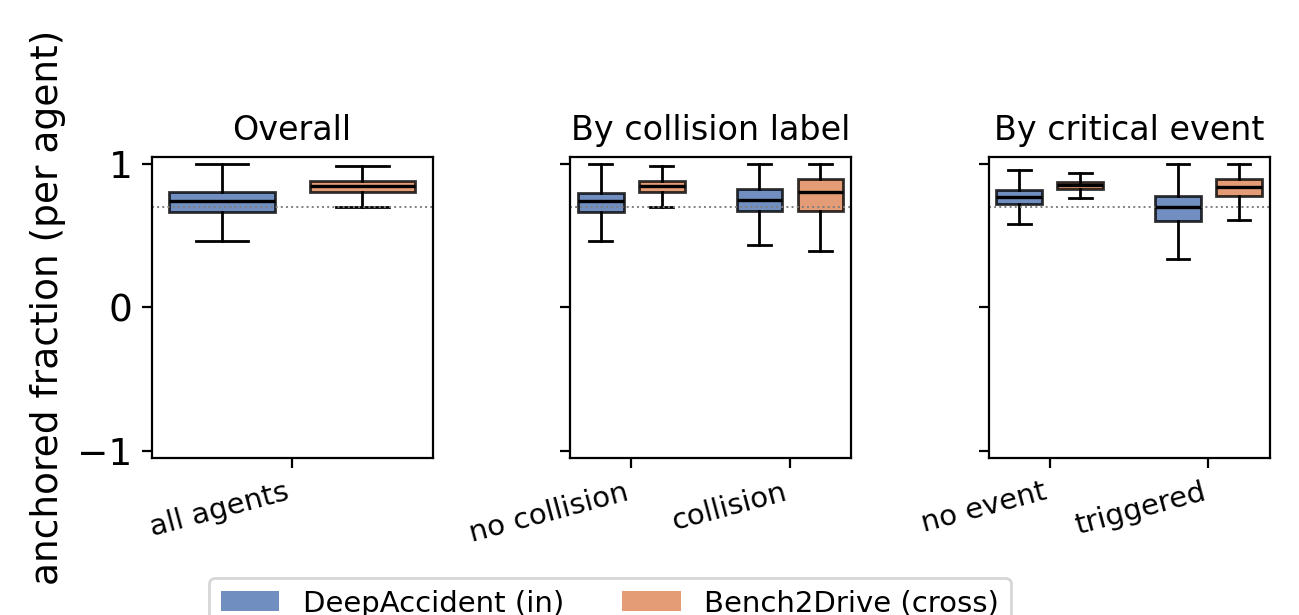
\includegraphics[width=3.3in]{figures/anchored_fraction_distribution.png}
\caption{Per-agent anchored-fraction distribution (DeepAccident in-domain,
Bench2Drive cross-domain; single seed), split by native/geometric collision
label and by whether the agent's ground-truth critical-event label
$T_{\mathrm{evt}}$ is finite within the horizon. Dotted line: the $70.1\%$
mean from Table~\ref{tab:interpretability_tradeoff}. Boxes clipped to
$[-1,1]$; outliers below $-1$ ($<0.22\%$ of agents, a ratio-blowup artifact
discussed in the text) are excluded from the plot but not from any
reported statistic.}
\label{fig:anchored_fraction_distribution}
\end{figure}

\subsection{Planner Comparison and Qualitative Analysis}
\label{sec:exp_planner_screening}

We test whether FutureRisk can rank planners the way collision rate does,
but with finer resolution. Four released Bench2Drive
planners~\cite{bench2drivezoo} are used: AD-MLP (kinematics only), TCP
(single front camera), and UniAD-Tiny and VAD-Base (surround-view BEV).
On each of $n=15$ eligible \emph{AccidentTwoWays} clips, the surrounding
agents' tracks are held fixed and only the ego box is replaced by the
planner's predicted path, interpolated onto CARM's time grid and
extrapolated at constant velocity beyond the planner's own horizon. All
trajectories are scored zero-shot by the DeepAccident-trained checkpoint.
Collision rate here means the fraction of clips with a geometric overlap
(Eq.~\eqref{eq:high_level_3d_ttc}).

Fig.~\ref{fig:planner_slope_chart} compares mean $R$ with collision rate
per planner. The two agree on TCP (safest) and AD-MLP (second), and
disagree on the remaining pair: mean $R$ ranks UniAD safer than VAD,
collision rate ranks VAD safer than UniAD. With $n=15$ the aggregate gap
is small ($0.382$ vs.\ $0.423$), and Fig.~\ref{fig:case_study_uniad_vs_vad}
locates almost all of it in a single clip where the two metrics disagree
by construction. In that clip, VAD's trajectory never overlaps any
agent's box within the 4\,s window, so the overlap test and the
closed-form margin register nothing ($m(t)=+\infty$, $r(t)\equiv0$,
panel~(a)). Its distance to one agent nevertheless shrinks monotonically
from $57.8$\,m to $3.4$\,m and is still closing at about $4$\,m/s when the
window ends (panel~(b2)); the critical-event hazard $q_k$ for that agent
rises steeply over the final bins (panel~(c)) and the trajectory scores
$R=0.975$. UniAD, in the same scenario, collides with a different agent
at $t=0.6$\,s (panel~(b1)) and scores $R=0.962$. Removing this clip
brings VAD's mean $R$ to $0.383$, level with UniAD's $0.382$: the
planner-level disagreement is not noise but one interaction that a
fixed-horizon overlap test cannot register until contact occurs. This is
the case the critical-event branch was built for
(Sec.~\ref{sec:carm_training}): the geometric target $y$ is $0$ by
construction whenever no overlap occurs, and it is the independently
supervised hazard $q_k$, read from the realized interaction rather than
from any overlap, that carries the signal here.

Fig.~\ref{fig:qualitative_per_timestep_comparison} shows per-frame scores
along the ego path for two DeepAccident instances: a near-miss (top; no
contact) and a collision that the geometric overlap test misses entirely
(bottom; native label confirms contact at $t=4.0$\,s). On the missed
collision, raw 3D-TTC is $0.0$ at all $41$ frames, the same fixed-horizon
blindness seen for VAD above. RSS and GSSM respond, but at other times
(RSS peaks at $0.552$ at $t=3.1$\,s, GSSM at $3.85$ at $t=3.6$\,s, in its
own unbounded units). FutureRisk is elevated at the confirmed contact
frame ($R=0.478$) and crosses $0.4$
XX frames % TODO: check figure
before contact. Its scale is bounded to $[0,1]$ and, through the
anchoring of Sec.~\ref{sec:exp_tradeoff}, stays tied to the physics
prior, which neither GSSM's unbounded intensity nor RSS's
collision-insensitive envelope offers. On the near-miss, all four methods
rise toward the closest-approach point without flagging a collision;
FutureRisk shows a transient spike at $t=0.3$\,s, early in the clip, and
settles to the same near-certain value within one frame. Under the
geometric overlap test both instances carry label $0$, one of them
wrongly; FutureRisk assigns them distinct, correctly ordered scores.

\begin{figure}[t]
\centering
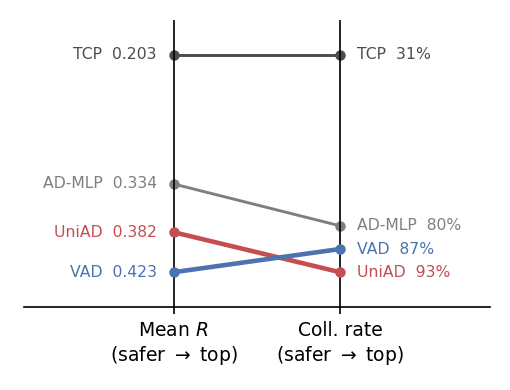
\includegraphics[width=2.5in]{figures/planner_slope_chart.png}
\caption{Planner ranking by mean $R$ (left) and by geometric collision
rate (right) over the same $n=15$ clips; on both axes, safer is higher.
Parallel lines (TCP, AD-MLP) mean the two metrics agree on the order;
crossing lines (UniAD, VAD) mean they disagree.}
\label{fig:planner_slope_chart}
\end{figure}


\begin{figure*}[t]
\centering
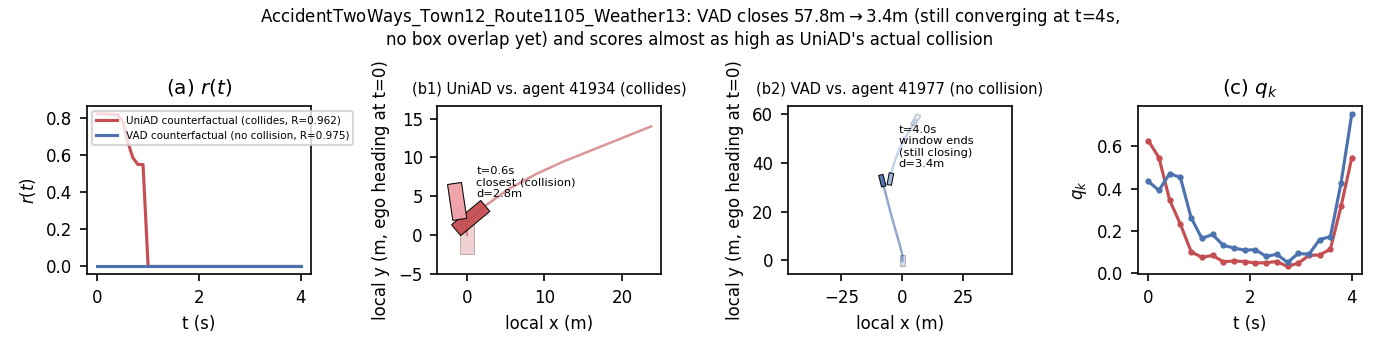
\includegraphics[width=7.0in]{figures/case_study_uniad_vs_vad.png}
\caption{One AccidentTwoWays scenario (Route~1105) under UniAD (red) and
VAD (blue). UniAD collides with one agent at $t=0.6$\,s ($R=0.962$). VAD
never overlaps any agent's box within the 4\,s window, yet closes on
another agent from $57.8$\,m to $3.4$\,m and is still approaching at about
$4$\,m/s when the window ends ($R=0.975$). (a) Closed-form per-frame risk
$r(t)$ (Eq.~\eqref{eq:continuous_risk}): nonzero for UniAD, zero for VAD.
(b1)/(b2) Bird's-eye view of ego and agent paths in each ego's local frame
at $t=0$; light boxes mark footprints at $t=0$, solid boxes at the moment
of interest (UniAD: contact; VAD: end of window). (c) Critical-event
hazard $q_k$ (Eq.~\eqref{eq:event_time_distribution}) for the agent each
case concerns.}
\label{fig:case_study_uniad_vs_vad}
\end{figure*}

\begin{figure}[t]
\centering
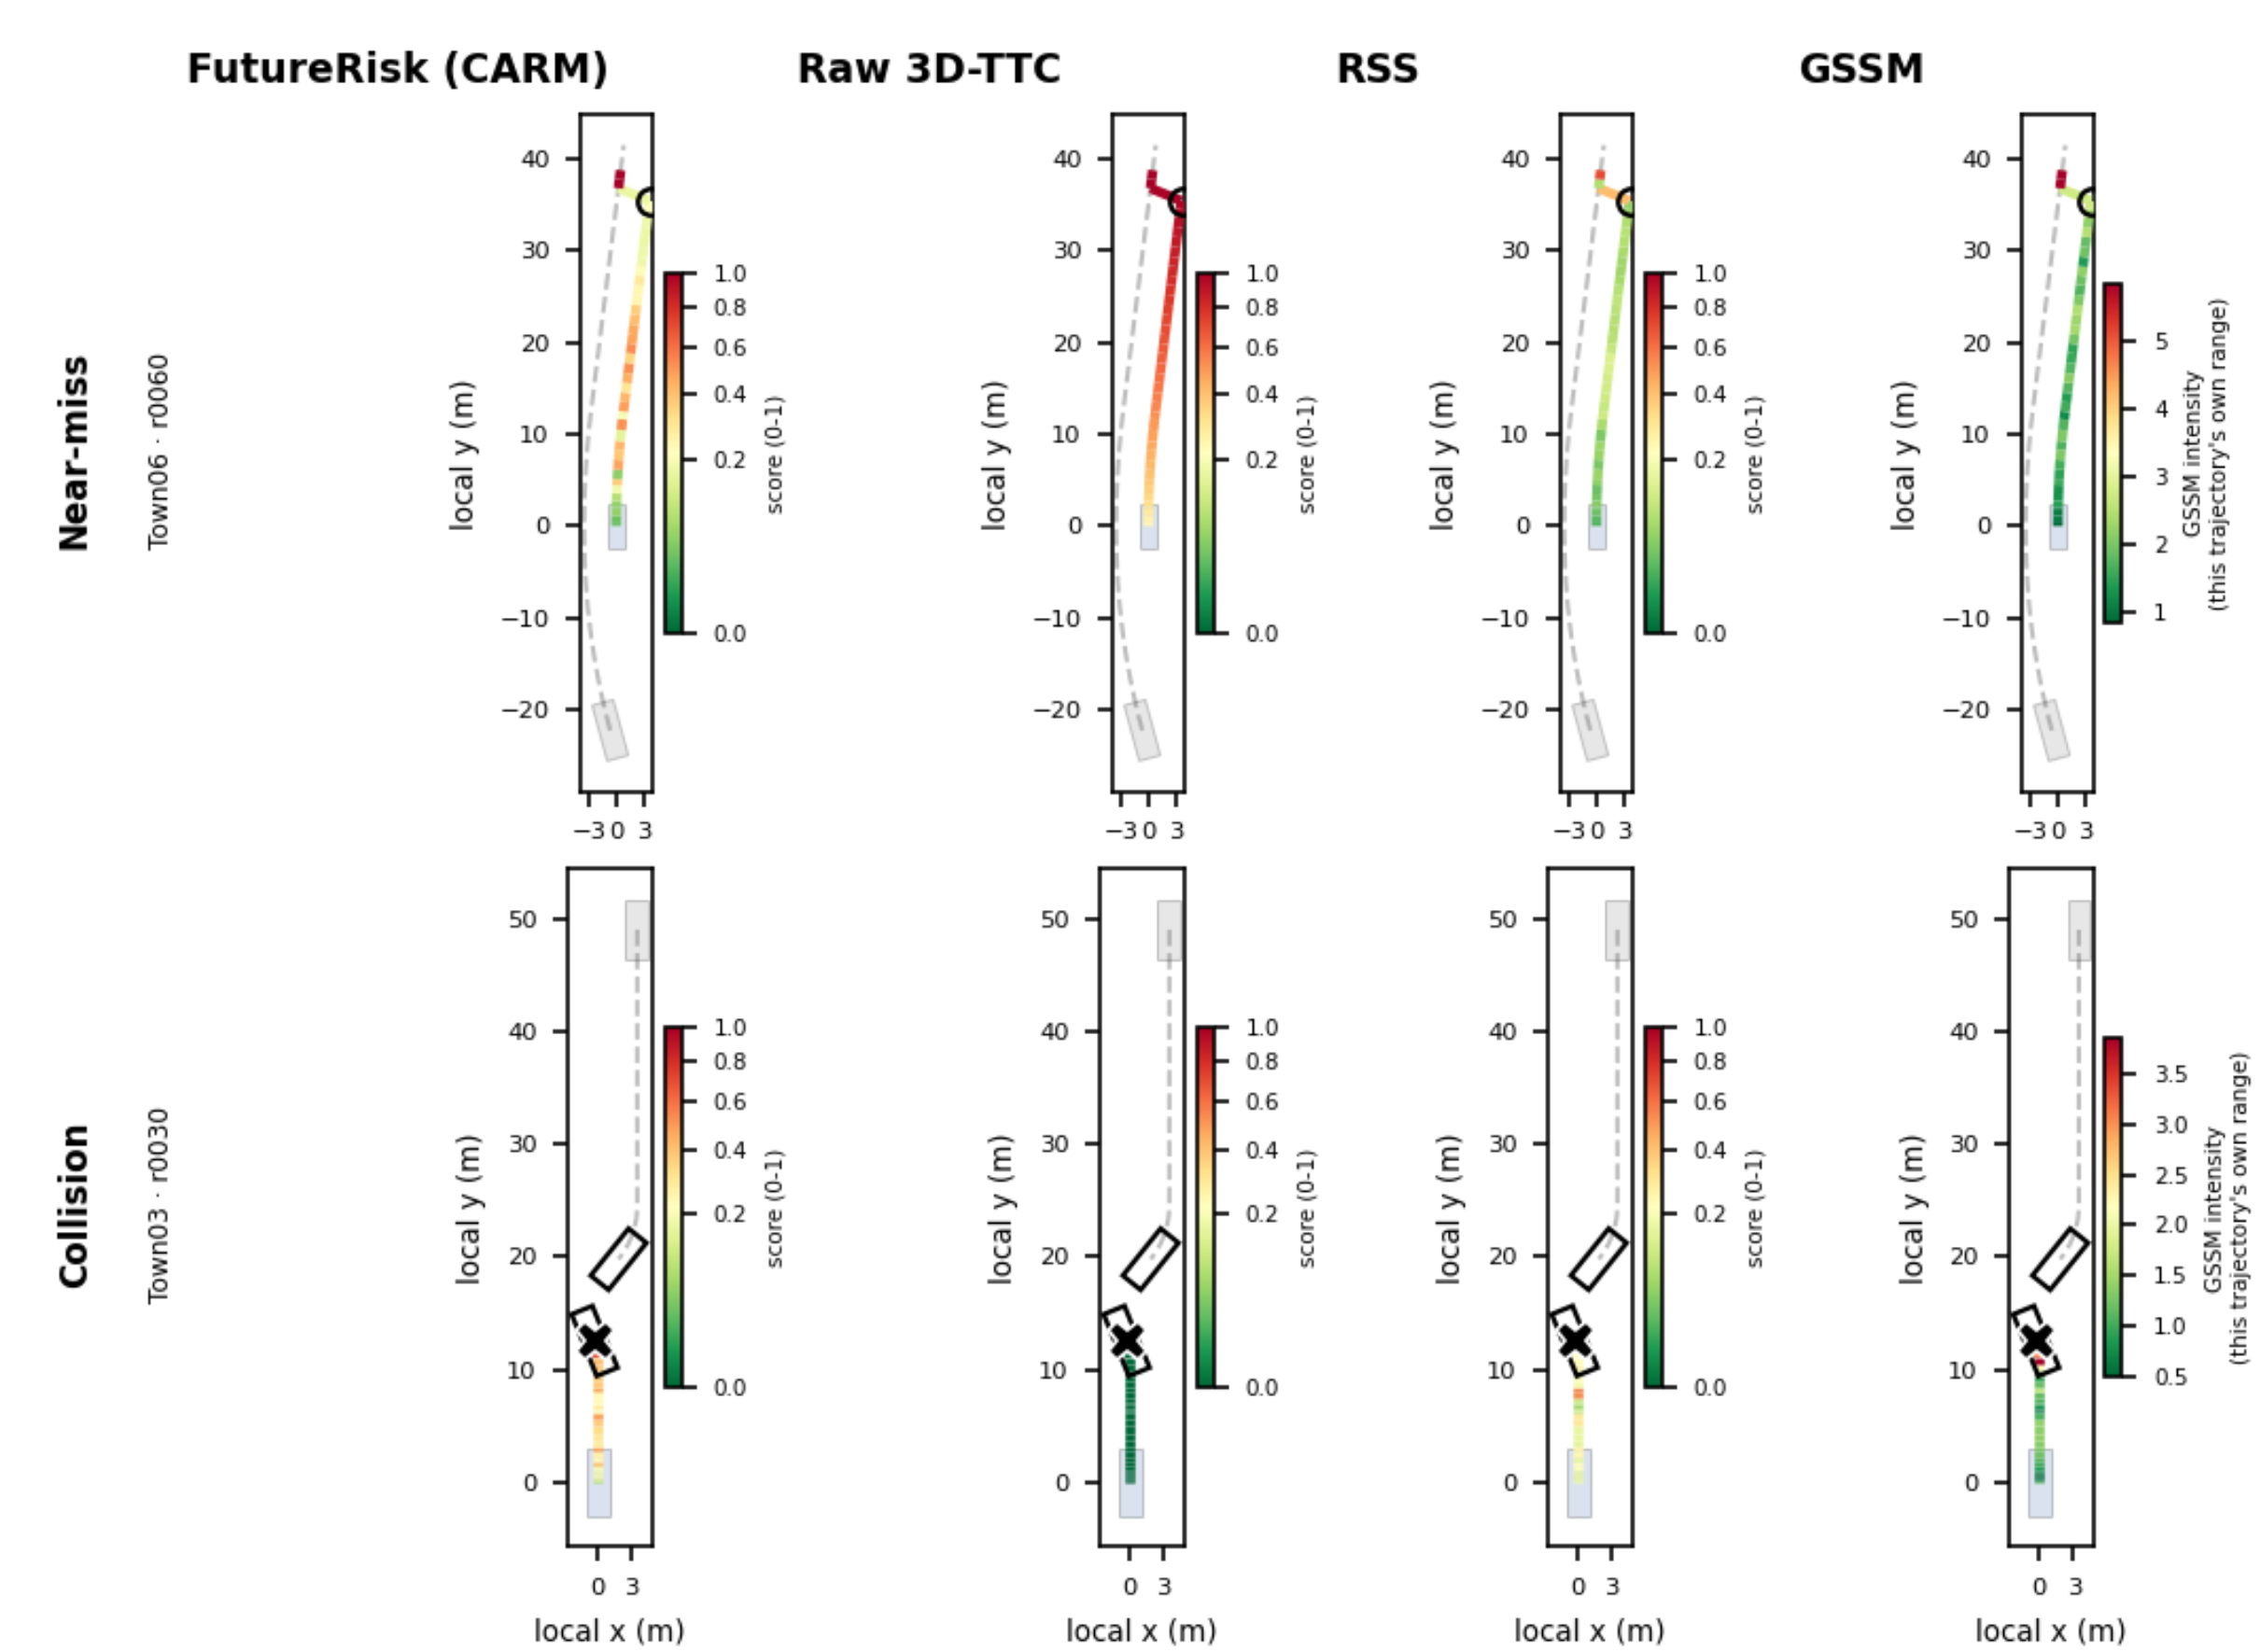
\includegraphics[width=3.50in]{figures/compare.drawio.png}
\caption{Per-timestep risk along the ego path for two real DeepAccident
instances (rows) under four methods (columns): a near-miss safely avoided
(top; native collision label $=0$) and a collision missed entirely by the
fixed-horizon geometric criterion (bottom; native collision label $=1$,
contact at $t=4.0$s). Path color is that method's own per-frame score
(green=low, red=high); FutureRisk, RSS, and raw 3D-TTC share one fixed
$[0,1]$ color scale, while GSSM's unbounded intensity is normalized to
each row's own observed range (its own colorbar). Gray dashed path is the
interacting agent; \textsf{X} marks the native-confirmed collision
contact; \textsf{o} marks the closest-approach frame on the near-miss row,
where no collision occurs.}
\label{fig:qualitative_per_timestep_comparison}
\end{figure}



\begin{figure}[t]
\centering
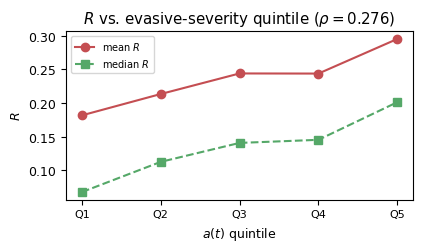
\includegraphics[width=2.7in]{figures/severity_bins.png}
\caption{Mean and median $R$ within each quintile of the evasive-severity
proxy $a(t)$, collision-free DeepAccident test instances ($n=6630$).
Both increase with severity; Spearman $\rho=0.276$ over all instances.}
\label{fig:severity_bins}
\end{figure}


\subsection{Perturbation Sweep and Hyperparameter Sensitivity}
\label{sec:exp_sensitivity}

\noindent\textbf{Perturbation sweep.}
Starting from a real DeepAccident collision, we shift the ego path
laterally (perpendicular to its per-frame heading) from $\delta=0$, where
it collides, to $\delta=6$\,m, where it passes with ample room, sampling
$55$ offsets and recomputing $R$, raw 3D-TTC, and PET at each
(Fig.~\ref{fig:perturbation_sweep}). The two rule-based scores are step
functions of $\delta$: raw 3D-TTC drops from $1.0$ to $0.0$ between two
adjacent offsets $0.02$\,m apart at the overlap boundary
($\delta\approx2.15$\,m), and PET does the same later
($\delta\approx5.1$--$5.4$\,m). $R$ moves smoothly across the whole
range; its largest change between adjacent offsets is $0.019$ and its
total variation is $0.19$. What the sweep compares is how far each score
moves when the trajectory moves a little: $R$ moves a little, and each
rule-based score moves its full scale at one offset.

\noindent\textbf{Hyperparameter sensitivity.}
The transition width $T_m$ in Eq.~\eqref{eq:continuous_risk} rescales the
margin monotonically, so it cannot change any ranking of
$y_{\mathrm{analytic}}$; we checked this on all $8279$ DeepAccident
instances (Kendall's $\tau=1$ between $T_m\in\{0.5,2.0\}$ and
$T_m=1.0$). The only way $T_m$ reaches CARM is through the training
target. When we retrain over $T_m\in\{0.5,1.0,2.0\}$ and critical-event
percentile $\{90,95,99\}$, at a reduced budget of $12$ Stage-1 and $6$
Stage-2 epochs, in-domain AUROC across the nine settings varies by at
most $0.019$ ($0.735$--$0.754$).

% \subsection{Binned Severity, Perturbation Sweep, and Hyperparameter Sensitivity}

% \textbf{Parametric perturbation sweep} (Fig.~\ref{fig:perturbation_sweep}):
% from a real DeepAccident collision, we shift ego's path laterally
% (perpendicular to per-frame heading) from $\delta=0$ (colliding) past
% the collision boundary to $\delta=6$m (clearly safe), $55$ steps,
% recomputing $R$, raw 3D-TTC, and PET at each. Raw 3D-TTC steps from
% $1.0$ to $0.0$ within a single $0.02$m step at the boundary
% ($\delta\approx2.15$m; total variation $=1.0$, the full scale); PET
% jumps similarly, later ($\delta\approx5.1$--$5.4$m); $R$ instead
% decreases smoothly (max step change $=0.019$, total variation $=0.19$).

\begin{figure}[t]
\centering
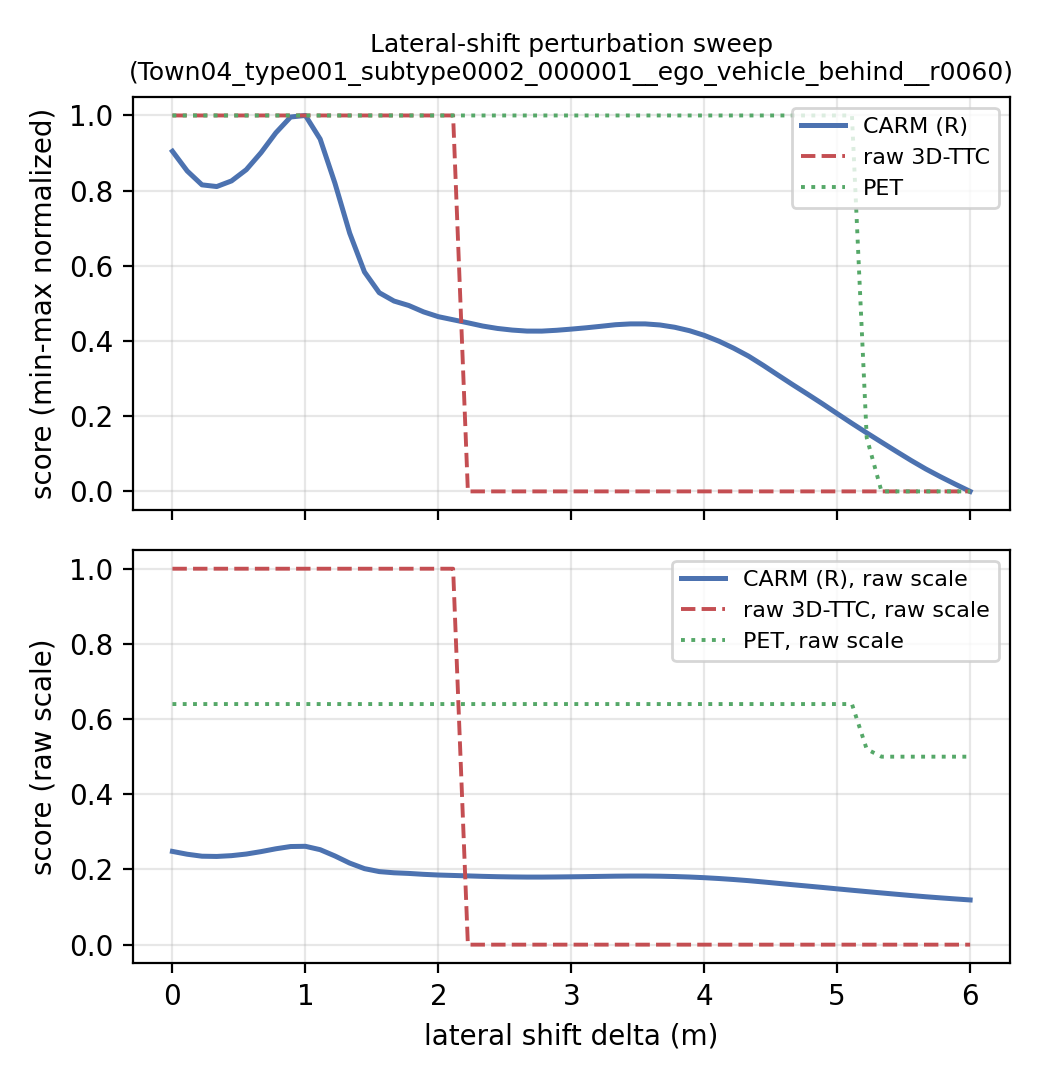
\includegraphics[width=2.6in]{figures/perturbation_sweep.png}
\caption{$R$, raw 3D-TTC, and PET as the ego path of one DeepAccident
collision instance is shifted laterally by $\delta$ (top: each score
min--max normalized; bottom: raw scale). Raw 3D-TTC and PET each jump
from one extreme to the other at a single offset; $R$ changes smoothly
throughout.}
\label{fig:perturbation_sweep}
\end{figure}

% \textbf{Hyperparameter sensitivity}: we confirm analytically and
% numerically, on all $8279$ cached DeepAccident instances, that $T_m$
% cannot affect any ranking metric of $y_{\mathrm{analytic}}$ by
% construction (monotonic rescaling preserves order): Kendall's $\tau$
% between $T_m\in\{0.5,2.0\}$ and $T_m=1.0$ rankings is exactly
% $1.000000$. Genuine sensitivity can only come from retraining: across
% the full $T_m\times\theta_{d,c}$-percentile grid
% ($\{0.5,1.0,2.0\}\times\{90,95,99\}$, each at a reduced $12$+$6$-epoch
% budget), in-domain AUROC stays within $0.735$--$0.754$, but the
% resulting ranking, relative to default, shows only moderate stability.



\balance
\begin{thebibliography}{99}
\scriptsize

\bibitem{hamidaoui2025survey}
M. Hamidaoui, M. Z. Talhaoui, M. Li, M. A. Midoun, S. Haouassi, D. E. Mekkaoui, A. Smaili, A. Cherraf, and F. Z. Benyoub,
\newblock “Survey of Autonomous Vehicles’ Collision Avoidance Algorithms,”
\newblock \emph{Sensors}, vol. 25, no. 2, p. 395, 2025.

\bibitem{jiang2025interactive}
J. Jiang, Z. Liu, H. Cheng, Z. Han, Z. Ke, Y. Wang, Q. Xu, and J. Wang,
\newblock ``Interactive Risk (IR): An Omnidirectional Safety Metric of CAVs Based on Multimodal Trajectory Prediction and Driving Risk Field,''
\newblock \emph{Accident Analysis \& Prevention}, vol. 222, p. 108228, 2025.

\bibitem{cui2025unified}
C. Cui, B. An, L. Li, X. Qu, and W. Li,
\newblock ``A Unified Risk Metric for Freeway Vehicles Based on the Spatio-Temporal Overlap Probability of Predicted Positions,''
\newblock \emph{Accident Analysis \& Prevention}, vol. 217, p. 108059, 2025.

\bibitem{westhofen2023criticality}
L. Westhofen, C. Neurohr, T. Koopmann, \emph{et al.},
\newblock ``Criticality Metrics for Automated Driving: A Review and Suitability Analysis of the State of the Art,''
\newblock \emph{Archives of Computational Methods in Engineering}, vol. 30, pp. 1--35, 2023.

\bibitem{montali2023wosac}
N. Montali, J. Lambert, P. Mougin, A. Kuefler, N. Rhinehart, M. Li, C. Gulino, T. Emrich, Z. Yang, S. Whiteson, B. White, and D. Anguelov,
\newblock ``The Waymo Open Sim Agents Challenge,''
\newblock \emph{arXiv preprint arXiv:2305.12032}, 2023.

\bibitem{caesar2021nuplan}
H. Caesar, J. Kabzan, K. S. Tan, \emph{et al.},
\newblock ``NuPlan: A Closed-Loop ML-Based Planning Benchmark for Autonomous Vehicles,''
\newblock \emph{arXiv preprint arXiv:2106.11810}, 2021.

\bibitem{weng2020mprism}
B. Weng, S. J. Rao, E. Deosthale, S. Schnelle, and F. Barickman,
\newblock ``Model Predictive Instantaneous Safety Metric for Evaluation of Automated Driving Systems,''
\newblock in \emph{IEEE Intelligent Vehicles Symposium (IV)}, 2020.

\bibitem{wang2021review}
C. Wang, Y. Xie, H. Huang, and P. Liu,
\newblock ``A Review of Surrogate Safety Measures and Their Applications in Connected and Automated Vehicles Safety Modeling,''
\newblock \emph{Accident Analysis \& Prevention}, vol. 157, p. 106157, 2021.

\bibitem{arun2021systematic}
A. Arun, M. M. Haque, A. Bhaskar, S. Washington, and T. Sayed,
\newblock ``A Systematic Mapping Review of Surrogate Safety Assessment Using Traffic Conflict Techniques,''
\newblock \emph{Accident Analysis \& Prevention}, vol. 153, p. 106016, 2021.

\bibitem{lu2022learning}
J. Lu, O. Grembek, and M. Hansen,
\newblock ``Learning the Representation of Surrogate Safety Measures to Identify Traffic Conflict,''
\newblock \emph{Accident Analysis \& Prevention}, vol. 174, p. 106755, 2022.

\bibitem{shalevshwartz2017rss}
S. Shalev-Shwartz, S. Shammah, and A. Shashua,
\newblock ``On a Formal Model of Safe and Scalable Self-Driving Cars,''
\newblock \emph{arXiv preprint arXiv:1708.06374}, 2017.

\bibitem{li2024beyond}
S. Li, M. Anis, D. Lord, H. Zhang, Y. Zhou, and X. Ye,
\newblock ``Beyond 1D and Oversimplified Kinematics: A Generic Analytical Framework for Surrogate Safety Measures,''
\newblock \emph{arXiv preprint arXiv:2312.07019}, 2024.

\bibitem{deepaccident}
T. Wang, S. Kim, W. Ji, E. Xie, C. Ge, J. Chen, Z. Li, and P. Luo,
\newblock ``DeepAccident: A Motion and Accident Prediction Benchmark for V2X Autonomous Driving,''
\newblock \emph{Proceedings of the AAAI Conference on Artificial Intelligence}, vol. 38, no. 6, pp. 5599--5606, 2024.

\bibitem{bench2drivezoo}
Thinklab-SJTU,
\newblock ``Bench2DriveZoo: Training, Open-Loop, and Closed-Loop Evaluation Code for BEVFormer, UniAD, VAD, TCP, and AD-MLP in Bench2Drive,''
\newblock \url{https://github.com/Thinklab-SJTU/Bench2DriveZoo}, accessed 2026. Released checkpoint used: \texttt{admlp\_b2d.ckpt} (\texttt{tcp/admlp} branch).

\bibitem{bench2drive}
X. Jia, Z. Yang, Q. Li, Z. Zhang, J. Bu, and J. Yan,
\newblock ``Bench2Drive: Towards Multi-Ability Benchmarking of Closed-Loop End-to-End Autonomous Driving,''
\newblock \emph{Advances in Neural Information Processing Systems (NeurIPS), Datasets and Benchmarks Track}, 2024.

\bibitem{jiao2026gssm}
Y. Jiao, S. C. Calvert, S. van Cranenburgh, and H. van Lint,
\newblock ``Learning Collision Risk from Naturalistic Driving with Generalised Surrogate Safety Measures,''
\newblock \emph{Nature Machine Intelligence}, 2026, \emph{arXiv preprint arXiv:2505.13556}. Code: \url{https://github.com/Yiru-Jiao/GSSM}. Released checkpoint used: \texttt{SafeBaseline/current+acc/model\_final\_71epoch.pth} (kinematics-only encoder, zero-shot, no fine-tuning).

\end{thebibliography}

\end{document}

\end{thebibliography}

\end{document}
